% !TEX root = ../main.tex
\section{Results and Conclusions}
\label{14::results_and_conclusions}
    The FMT efficiency is discussed in the first section, including a brief study of it.
    Then, the second section delves into the acceptance correction results, based on the methodology described in Section \ref{13.40::acceptance_correction}.
    Following that, the study results are discussed in detail, and the conclusions of the study follow shortly thereafter.

    % Run configuration.
    All Figures in this section that show results for data are from RG-F run 12016.
    For this run, a gas H2 target was used.
    The beam energy was set to $10.4$ GeV, and the luminosity to $250$ nA.
    The solenoid field was set to an inbending polarity ($-0.75$), and the torus to its regular polarity of $-1$.
    The run has a total of $10,046,225$ events.

    % !TEX root = ../main.tex
\subsection{FMT Efficiency}
\label{14.10::fmt_efficiency}
    % Low FMT efficiency + list sources.
    Compared to the alignment work described in section \ref{12::fmt_alignment_and_reconstruction}, a low FMT is observed in this analysis.
    This is evident in figure \ref{fig::14.10::vz_012933}.
    Upon inspection, three causes can be attributed to this: the application of incorrect alignment constants, a geometry effect, and a general FMT offline reconstruction issue.

    \begin{figure}[b!]
        \centering\frame{
        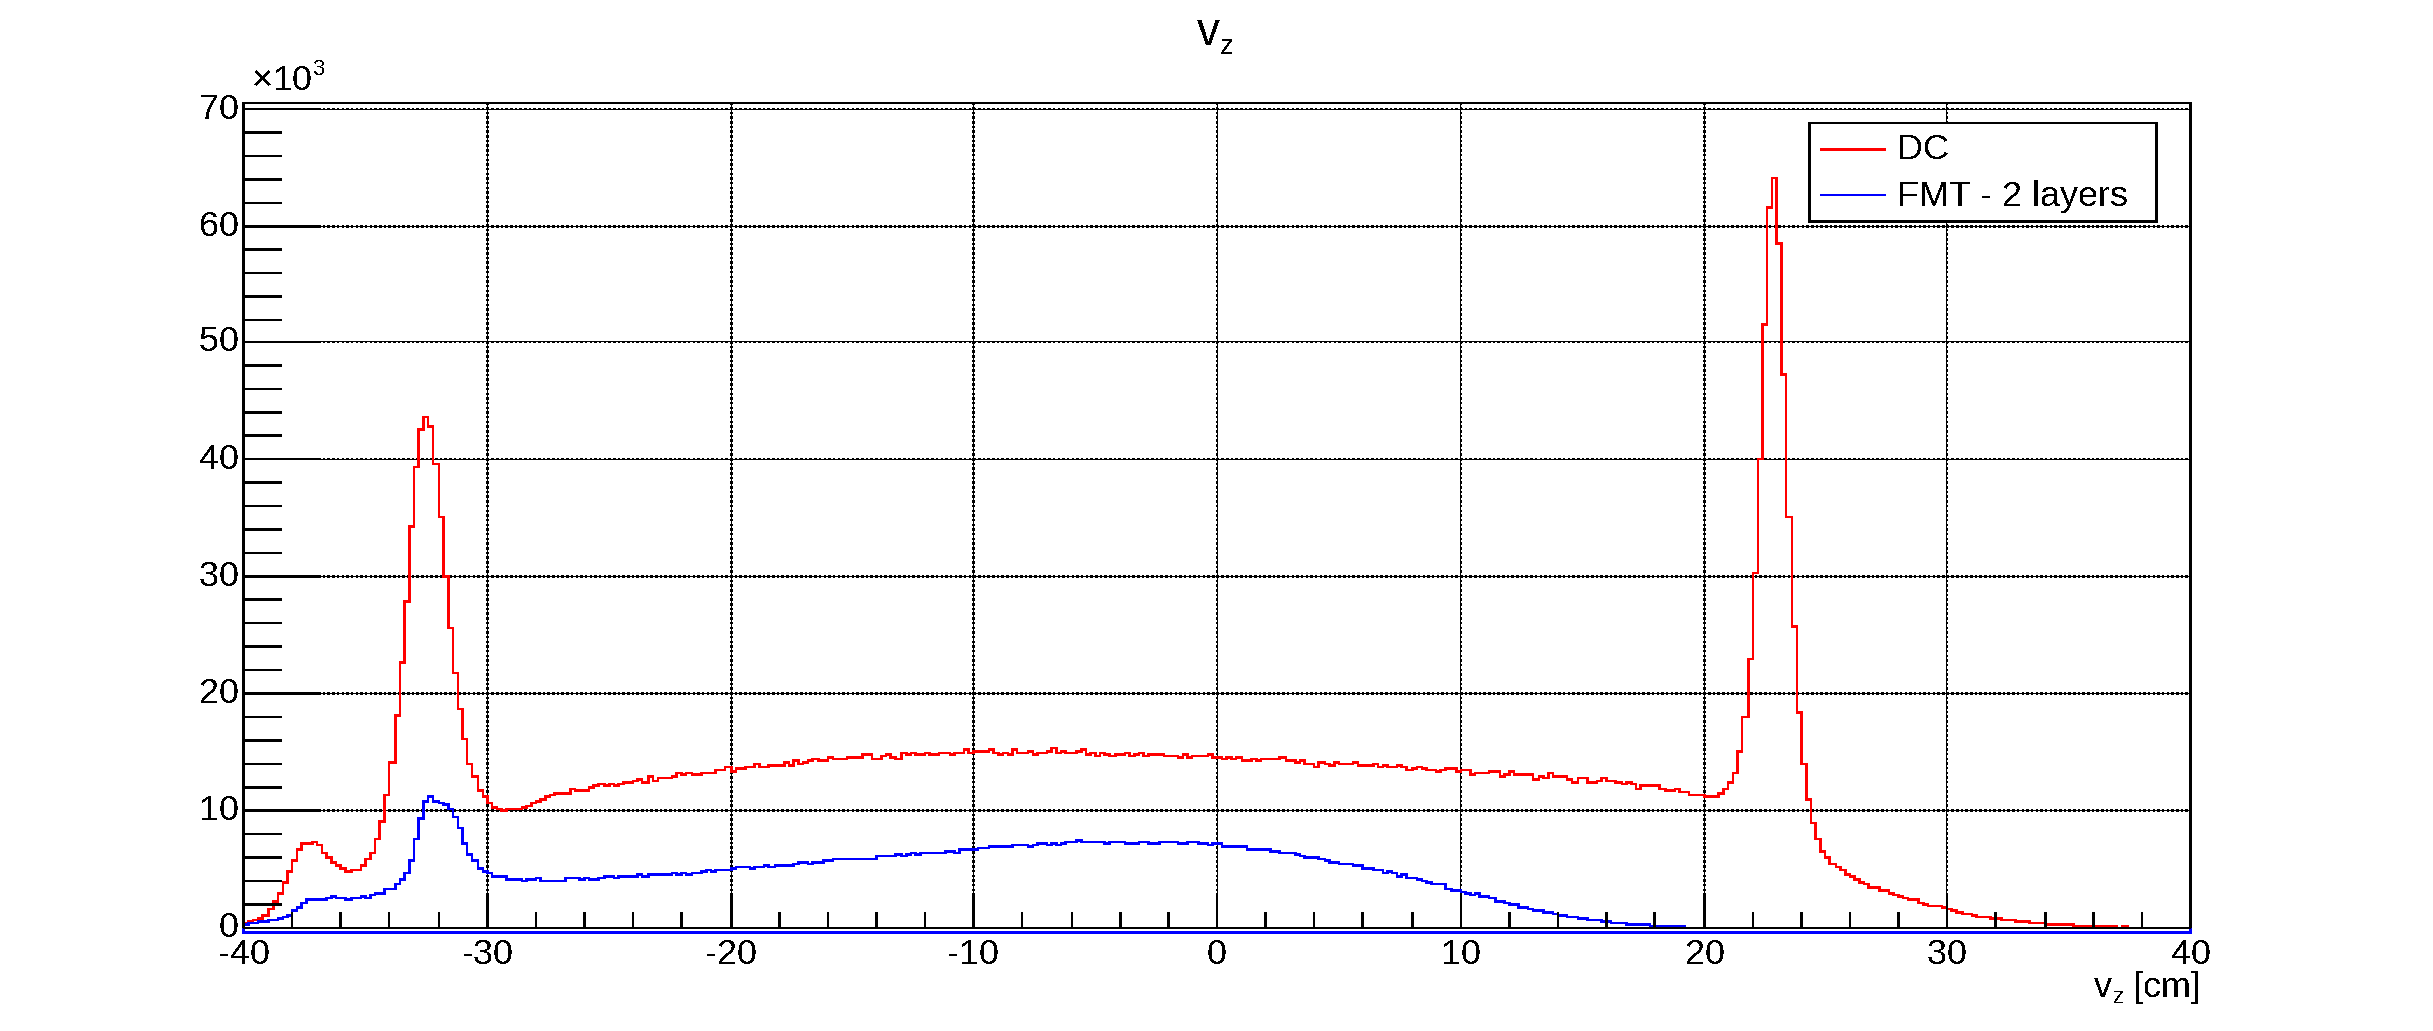
\includegraphics[width=\textwidth]{10vz_012933.pdf}}
        \caption[$v_z$ for DC and FMT, run 12933]{$v_z$ for DC (in red) and FMT (in blue). Summer 2020 data, run 12933. The wide peaks in FMT suggest an uncorrected misalignment.}
        \label{fig::14.10::vz_012933}
    \end{figure}

    % !TEX root = ../main.tex
\subsubsection{Alignment Effect}
\label{14.11::alignment_effect}
    % Introduction: The problem.
    The RG-F experiment's data is divided based on the season over which runs take place, thus there is Spring 2020 and Summer 2020 data.
    Based on the run group's guidelines, it is recommended to use Summer data, as it has seen more calibration than the Spring data.
    However, this calibration work hasn't included the FMT detector, and a strong misalignment effect is observed.

    % Cause of the problem.
    By simple visual inspection, two peaks can be clearly seen between $z = -36$ cm and $z = -30$ cm in figure \ref{fig::12.41::dc_vs_fmt_vz_11983}.
    These peaks are merged in figure \ref{fig::14.10::vz_012933}.
    As discussed in section \ref{12::fmt_alignment_and_reconstruction}, this issue comes from a lack of correction for FMT misalignments.

    % Solution.
    The simplest solution is to use Spring data.
    While more work has been put on Summer data, it mainly pertains to the central detector; unrelated to this analysis.
    Figure \ref{fig::14.11::vz_012016} shows the same $v_z$ plot from Spring 2020 run 12016.
    Both peaks are clearly visible in this plot, suggesting that misalignments are properly accounted for in the run.

    \begin{figure}[t!]
        \centering\frame{
        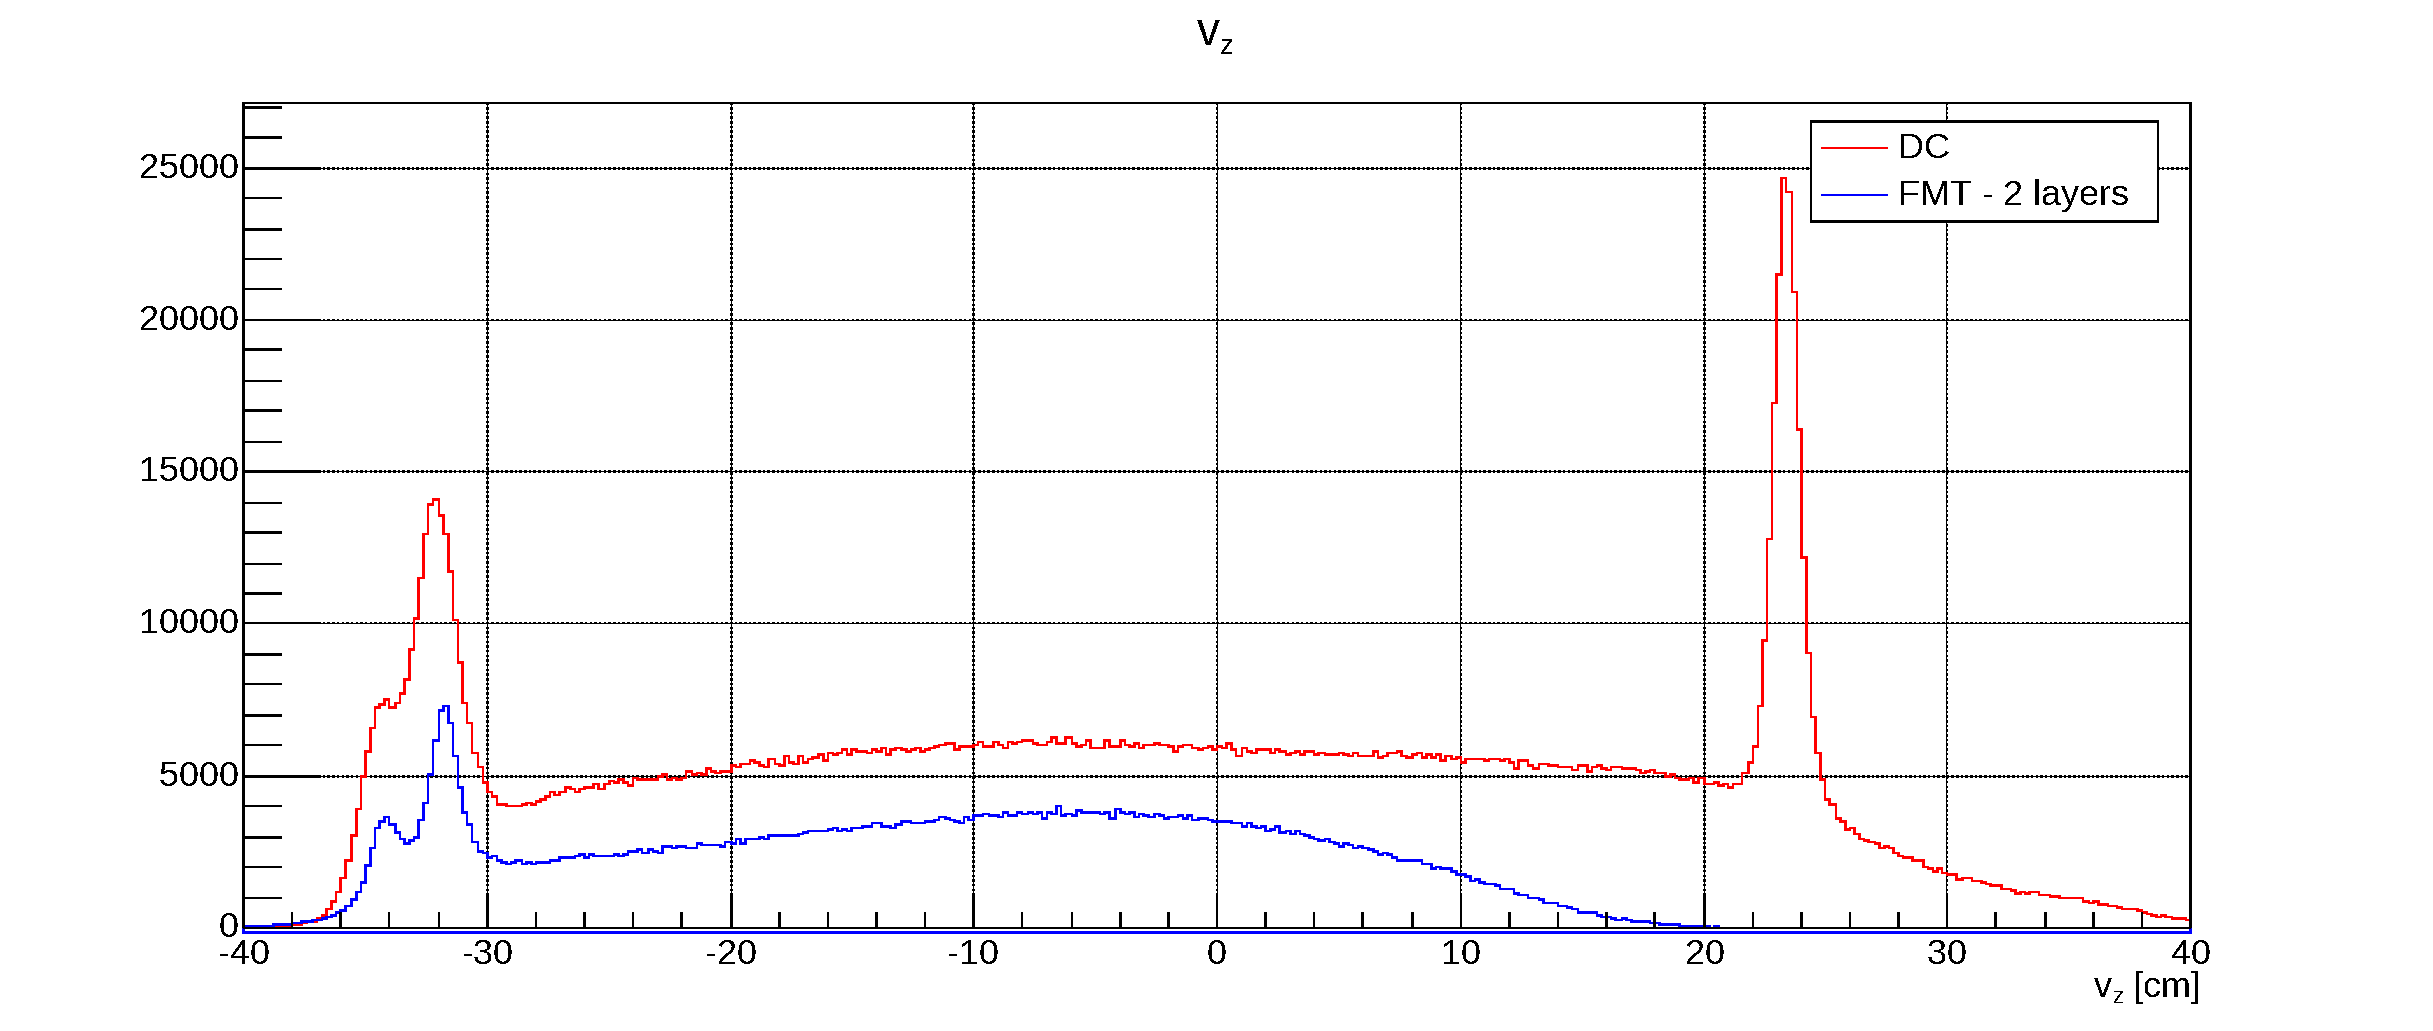
\includegraphics[width=\textwidth]{11vz_012016.pdf}}
        \caption[$v_z$ for DC and FMT, run 12016]{$v_z$ for DC (in red) and FMT (in blue). Spring 2020 data, run 12016. The upstream twin peaks can be clearly distinguished, suggesting a correct misalignment correction.}
        \label{fig::14.11::vz_012016}
    \end{figure}

    % !TEX root = ../main.tex
\subsubsection{Geometry Effect}
\label{sssec::geometry_effect}
    % The effect has already been presented and discussed before, so we're brief.
    This problem is already discussed in detail in section \ref{sssec::geometry_effect}.
    As a quick reminder, FMT sits at $z \approx 26$ cm, and it naturally performs poorly for targets to close to it.
    We can measure the strength of this effect by applying the geometry cut given by equation \eqref{eq::12.42::fmt_geometry_cut} to both DC and FMT tracks.
    Figure \ref{fig::vz_012016_geomcut} the effect of the cut when applied on figure \ref{fig::vz_012016}.
    Its effect on a $v_z$ vs $\theta$ plot can be seen on figure \ref{eq::12.42::vz_vs_theta}.

    Based on this cut and the FMT $z$ position, subsequent plots will be constrained to the range $-30 \text{[cm]} < v_z < 20 \text{[cm]}$.

    \begin{figure}[h!]
        \centering\frame{
        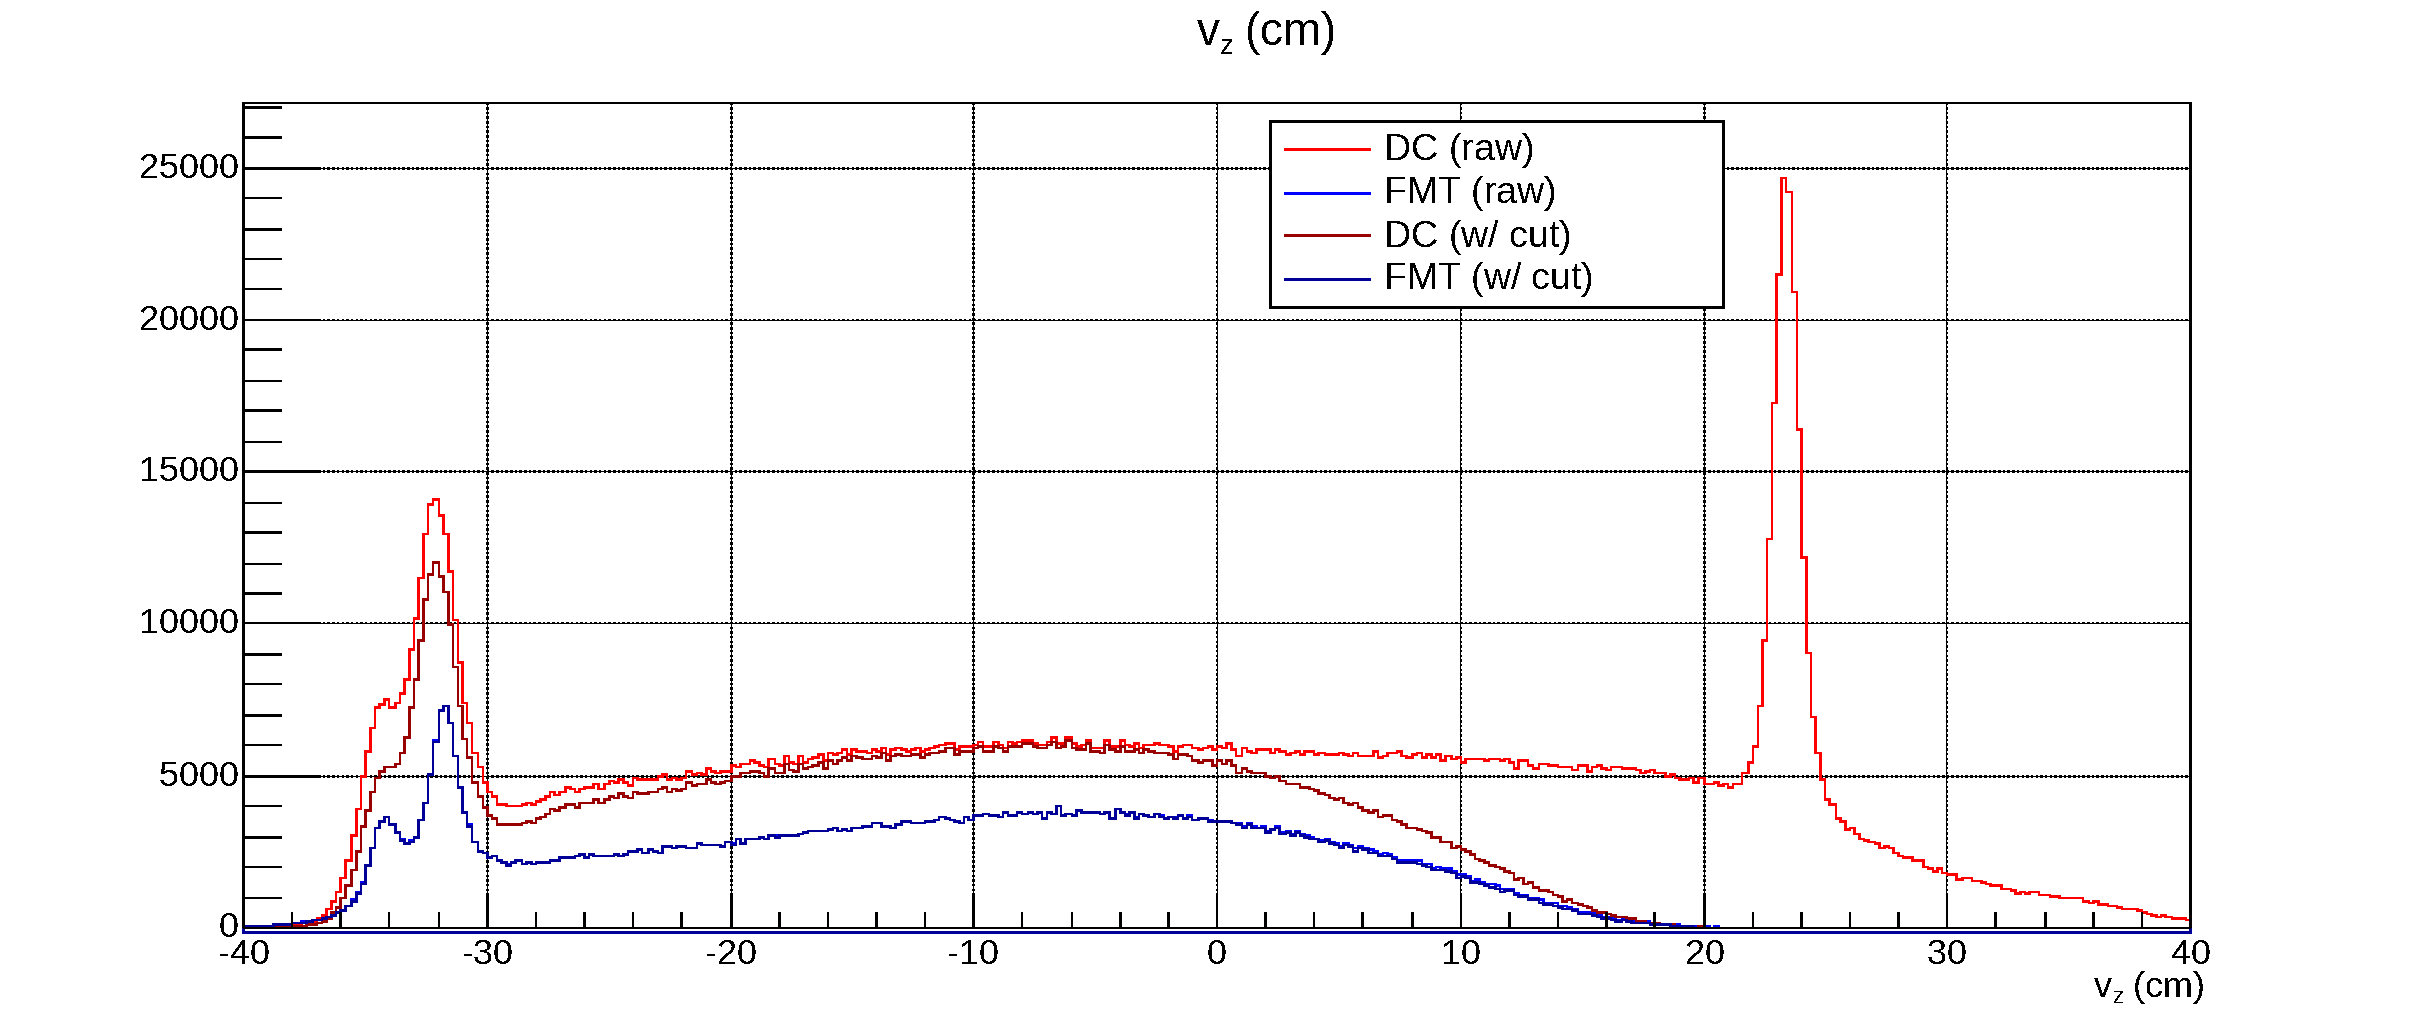
\includegraphics[width=\textwidth]{12vz_012016_geomcut.pdf}}
        \caption[$v_z$ for DC and FMT, w/ and w/out the geometry cut, run 12016]{$v_z$ for DC without the geometry cut (in red), with it (in dark red), for FMT without it (in blue), and with it (in dark blue). Spring 2020 data, run 12016. The effect is very clear on DC tracks, yet it almost doesn't affect FMT tracks.}
        \label{fig::vz_012016_geomcut}
    \end{figure}

    % !TEX root = ../main.tex
\subsubsection{Reconstruction Effect}
\label{14.13::reconstruction_effect}
    Even after correcting for both the alignment and geometry issues, FMT still has a lower efficiency when compared to that found during alignment (compare figures \ref{fig::14.12::vz_012016_geomcut} with \ref{fig::12.43::dc_vs_fmt_vz_11983_corrected}).
    After some study, the effect was found not to be correlated to run number, beam energy, or beam luminosity.
    Based on this, we can discard it being caused by hardware issues or run conditions.

    Based on this, the logical conclusion is that the effect comes from a general issue in FMT offline reconstruction.
    Finding and fixing this would be a larger project than what's contemplated in the scope of this thesis, so it's left as future work.
    For the purposes of this analysis, we'll contempt ourselves with using a large number of events, minimising statistic deficiencies.

    % !TEX root = ../main.tex
\subsubsection{Efficiency Study}
\label{14.14::efficiency_study}
% --+ Integrated. +-------------------------------------------------------------
    With all these effects accounted for, we can proceed to study the efficiency in detail.
    First, if we define FMT efficiency as the percentage of DC tracks that get accepted by FMT, we get the results in Table \ref{tab::14.14::fmt_efficiency_study} for runs 12933 (Summer 2020) and 12016 (Spring 2020), as well as the simulation described in Section \ref{13.40::acceptance_correction}.

    \begin{table}[b]
        \begin{center}
            \begin{tabularx}{0.86\textwidth}{Xlcrrcrr}
                \toprule
                & & & \multicolumn{2}{c}{\textbf{Run 12933}} & & \multicolumn{2}{c}{\textbf{Run 12016}} \\
                                    &          & & \multicolumn{1}{c}{raw} & \multicolumn{1}{c}{w/ cut} & & \multicolumn{1}{c}{raw} & \multicolumn{1}{c}{w/ cut} \\
                \midrule \midrule
                \textbf{$e^-$}      & 2 layers & & $25.1 \pm 1.5$ & $37.5 \pm 0.7$ & & $32.7 \pm 2.5$ & $53.7 \pm 0.8$ \\
                                    & 3 layers & & $ 5.6 \pm 2.7$ & $ 8.5 \pm 1.7$ & & $ 9.9 \pm 6.3$ & $16.4 \pm 3.6$ \\
                \midrule
                \textbf{$e^-\pi^+$} & 2 layers & & $ 6.5 \pm 0.2$ & $13.7 \pm 0.9$ & & $11.1 \pm 0.2$ & $28.0 \pm 1.3$ \\
                                    & 3 layers & & $ 0.3 \pm 0.1$ & $ 0.7 \pm 0.4$ & & $ 1.0 \pm 0.1$ & $ 2.7 \pm 1.4$ \\
                \midrule
                \textbf{$e^-\pi^-$} & 2 layers & & $ 5.6 \pm 0.0$ & $14.2 \pm 1.0$ & & $ 8.9 \pm 0.4$ & $29.5 \pm 1.4$ \\
                                    & 3 layers & & $ 0.3 \pm 0.0$ & $ 0.7 \pm 0.5$ & & $ 0.9 \pm 0.3$ & $ 2.9 \pm 1.6$ \\
                \bottomrule
            \end{tabularx}
        \end{center}
        \caption[FMT efficiency study results]
        {Results of the FMT efficiency study performed in $\%$.}
        \label{tab::14.14::fmt_efficiency_study}
    \end{table}

    % --+ Error estimation +----------------------------------------------------
    To estimate the efficiency of one FMT layer and the associated errors for the two types of tracks, we define $P(L_n)$ as the probability of layer $n$ detecting a particle, with $1 \leq n \leq 3$.
    Assuming that all layers have the same efficiency, denoted as $E_1$,
    \begin{equation*}
        P(L_1) = P(L_2) = P(L_3) = E_1,
    \end{equation*}
    the efficiency $E_3$ for 3-layer tracks can be obtained using the probabilities $P(L_n)$ as follows
    \begin{align}
        E_3 &= P(L_1)P(L_2)P(L_3)
        \nonumber \\
        E_3 &= E_{1(3)}^3,
        \label{eq::14.14::efficiency3}
    \end{align}
    where $E_{1(3)}$ is the 1-layer efficiency estimated from 3-layer tracks.

    For 2-layer tracks, the efficiency $E_2$ can be obtained as
    \begin{align}
        E_2 &= P(L_1)P(L_2)\left(1 - P(L_3)\right)                \nonumber \\
             &\hspace{24pt} + P(L_2)P(L_3)\left(1 - P(L_1)\right) \nonumber \\
             &\hspace{24pt} + P(L_3)P(L_1)\left(1 - P(L_2)\right) \nonumber \\
             &\hspace{24pt} + P(L_1)P(L_2)P(L_3)                  \nonumber \\
        E_2 &= 3E_{1(2)}^2\left(1 - E_{1(2)}\right) + E_{1(3)}^3
            \nonumber \\
        E_2 &= 3E_{1(2)}^2 \cdot \left( 1 - E_{1(2)} \right) + E_3,
        \label{eq::14.14::efficiency2}
    \end{align}
    where $E_{1(2)}$ is the 1-layer efficiency estimated from 2-layer tracks.

    From \eqref{eq::14.14::efficiency3}, we can estimate $E_{1(3)}$ as
    \begin{equation}
        E_{1(3)} = \sqrt[3]{E_3}.
        \label{eq::14.14::efficiency1(3)}
    \end{equation}
    In contrast, $E_{1(2)}$ cannot be obtained explicitly from \eqref{eq::14.14::efficiency2}, but it can be estimated numerically.

    Using equations \eqref{eq::14.14::efficiency2} and \eqref{eq::14.14::efficiency1(3)}, we can estimate the weighted average efficiency $\xoverline{E_1}$ as
    \begin{equation*}
        \xoverline{E_1} = \frac{4E_{1(2)} + E_{1(3)}}{5},
    \end{equation*}
    where the weights are assigned based on the number of ways 2 and 3-layer tracks can be obtained, 4 and 1, respectively.

    From $\xoverline{E_1}$, we can estimate the errors on $E_{1(2)}$ and $E_{1(3)}$ as
    \begin{align*}
        \delta(E_{1(2)}) = |\xoverline{E_1} - E_{1(2)}|, \\
        \delta(E_{1(3)}) = |\xoverline{E_1} - E_{1(3)}|.
    \end{align*}

    To propagate these errors to the efficiencies $E_2$ and $E_3$, we use the variance formula
    \begin{equation*}
        \delta\left(f(x)\right) = \frac{\partial f(x)}{\partial x} \cdot \delta(x),
    \end{equation*}
    where $\delta(E_2)$, obtained from equation \eqref{eq::14.14::efficiency2}, is
    \begin{align*}
        \delta(E_2) &= \frac{\partial}{\partial E_{1(2)}} \left( 3E_{1(2)}^2 - 3E_{1(2)}^3 + E_{1(3)}^3 \right)
            \cdot \delta \left( E_{1(2)} \right) \\
        \delta(E_2) &= \left( 6E_{1(2)} - 9E_{1(2)}^2 \right) \cdot \delta \left( E_{1(2)} \right)
    \end{align*}
    and $\delta(E_3)$, obtained from equation \eqref{eq::14.14::efficiency3}, is
    \begin{align*}
        \delta(E_3) &= \frac{\partial}{\partial E_{1(3)}} \left( E_{1(3)}^3 \right) \cdot \delta \left( E_{1(3)} \right) \\
        \delta(E_3) &= 3E_{1(3)}^2 \cdot \delta \left( E_{1(3)} \right).
    \end{align*}

    A Python script was written to calculate $E_2$ and $E_3$ from each measurement shown in Table \ref{tab::14.14::fmt_efficiency_study}.
    The script is included in Appendix \ref{20.03::fmt_layer_efficiency_error_estimation}.
    The corresponding errors were obtained this way, and are included in the table.

    % --+ Conclusions drawn from table +----------------------------------------
    The table illustrates the positive impact of switching to Spring 2020 data and applying the geometry cut.
    The switch results in a $30.1\%$ increase in detected trigger electrons, as well as a $70.8\%$ increase for positive pions and a $58.9\%$ increase for negative pions.
    Furthermore, by applying the geometry cut based on $v_z$ and $\theta$, an additional $64.2\%$ increase in trigger electrons is achieved, resulting in a total increase of $113.9\%$.
    The pion yield experiences a substantial enhancement, with positive pions increasing by $150.2\%$ and negative pions increasing by $231.5\%$, resulting in a total increase of $330.8\%$ and $426.8\%$, respectively.

% --+ Separated. +--------------------------------------------------------------
    Next, we need to ensure that we are not introducing a systematic error by applying these corrections.
    To achieve this, we must investigate the effect of the geometry cut on different detected variables for electrons ($e^-$), positive pions ($e^-\pi^+$), and negative pions ($e^-\pi^-$).
    Based on the definition of the cut, we anticipate a strong correlation between efficiency and $v_z$ and $\theta$, and at most a weak correlation with $\phi$ and $p$.

    \begin{figure}
        % vz.
        \begin{subfigure}[b]{\textwidth}
            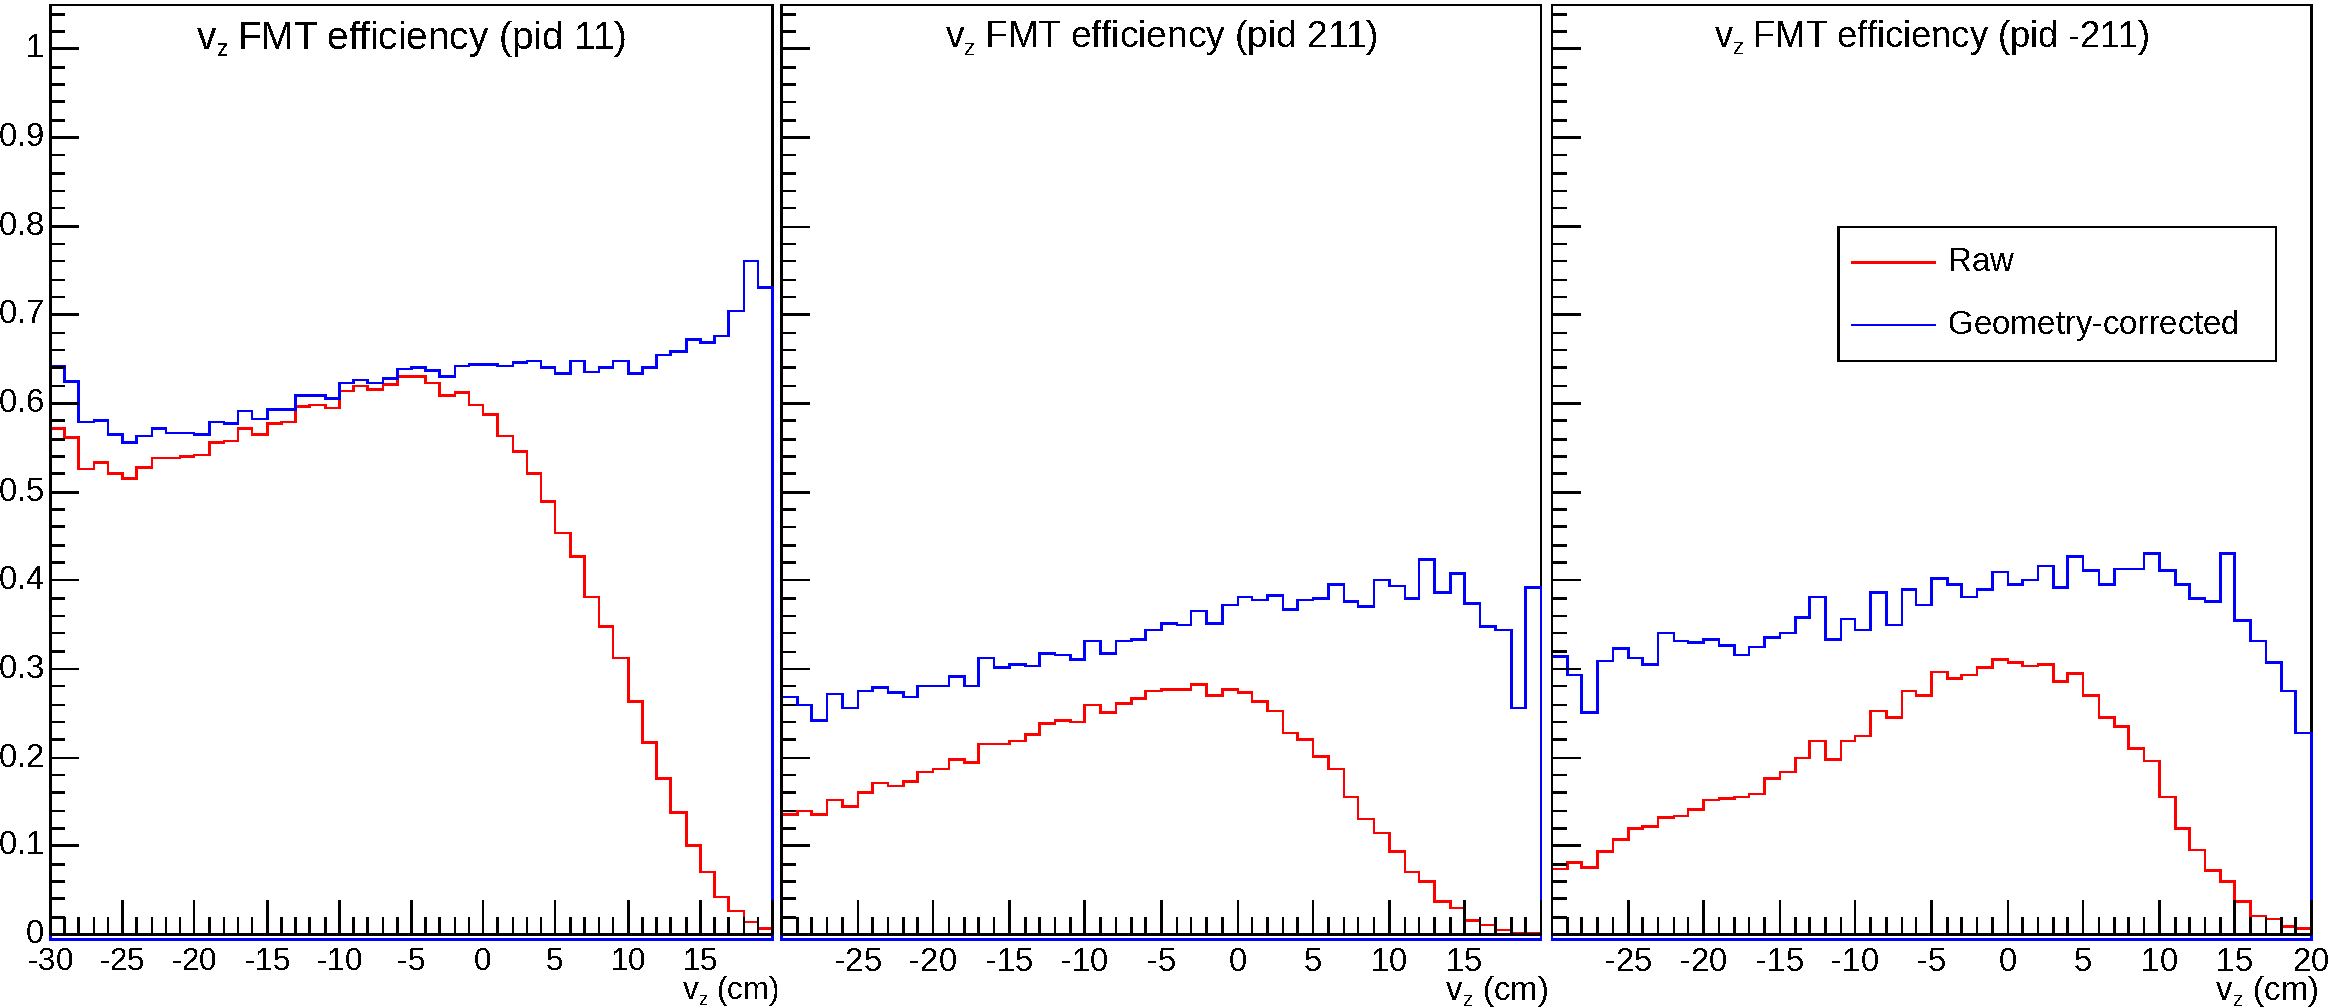
\includegraphics[width=\textwidth]{14vz_efficiency.pdf}
            \caption{$v_z$ FMT efficiency}
            \label{fig::14.14::fmt_efficiency_vz}
        \end{subfigure}
        % theta.
        \begin{subfigure}[b]{\textwidth}
            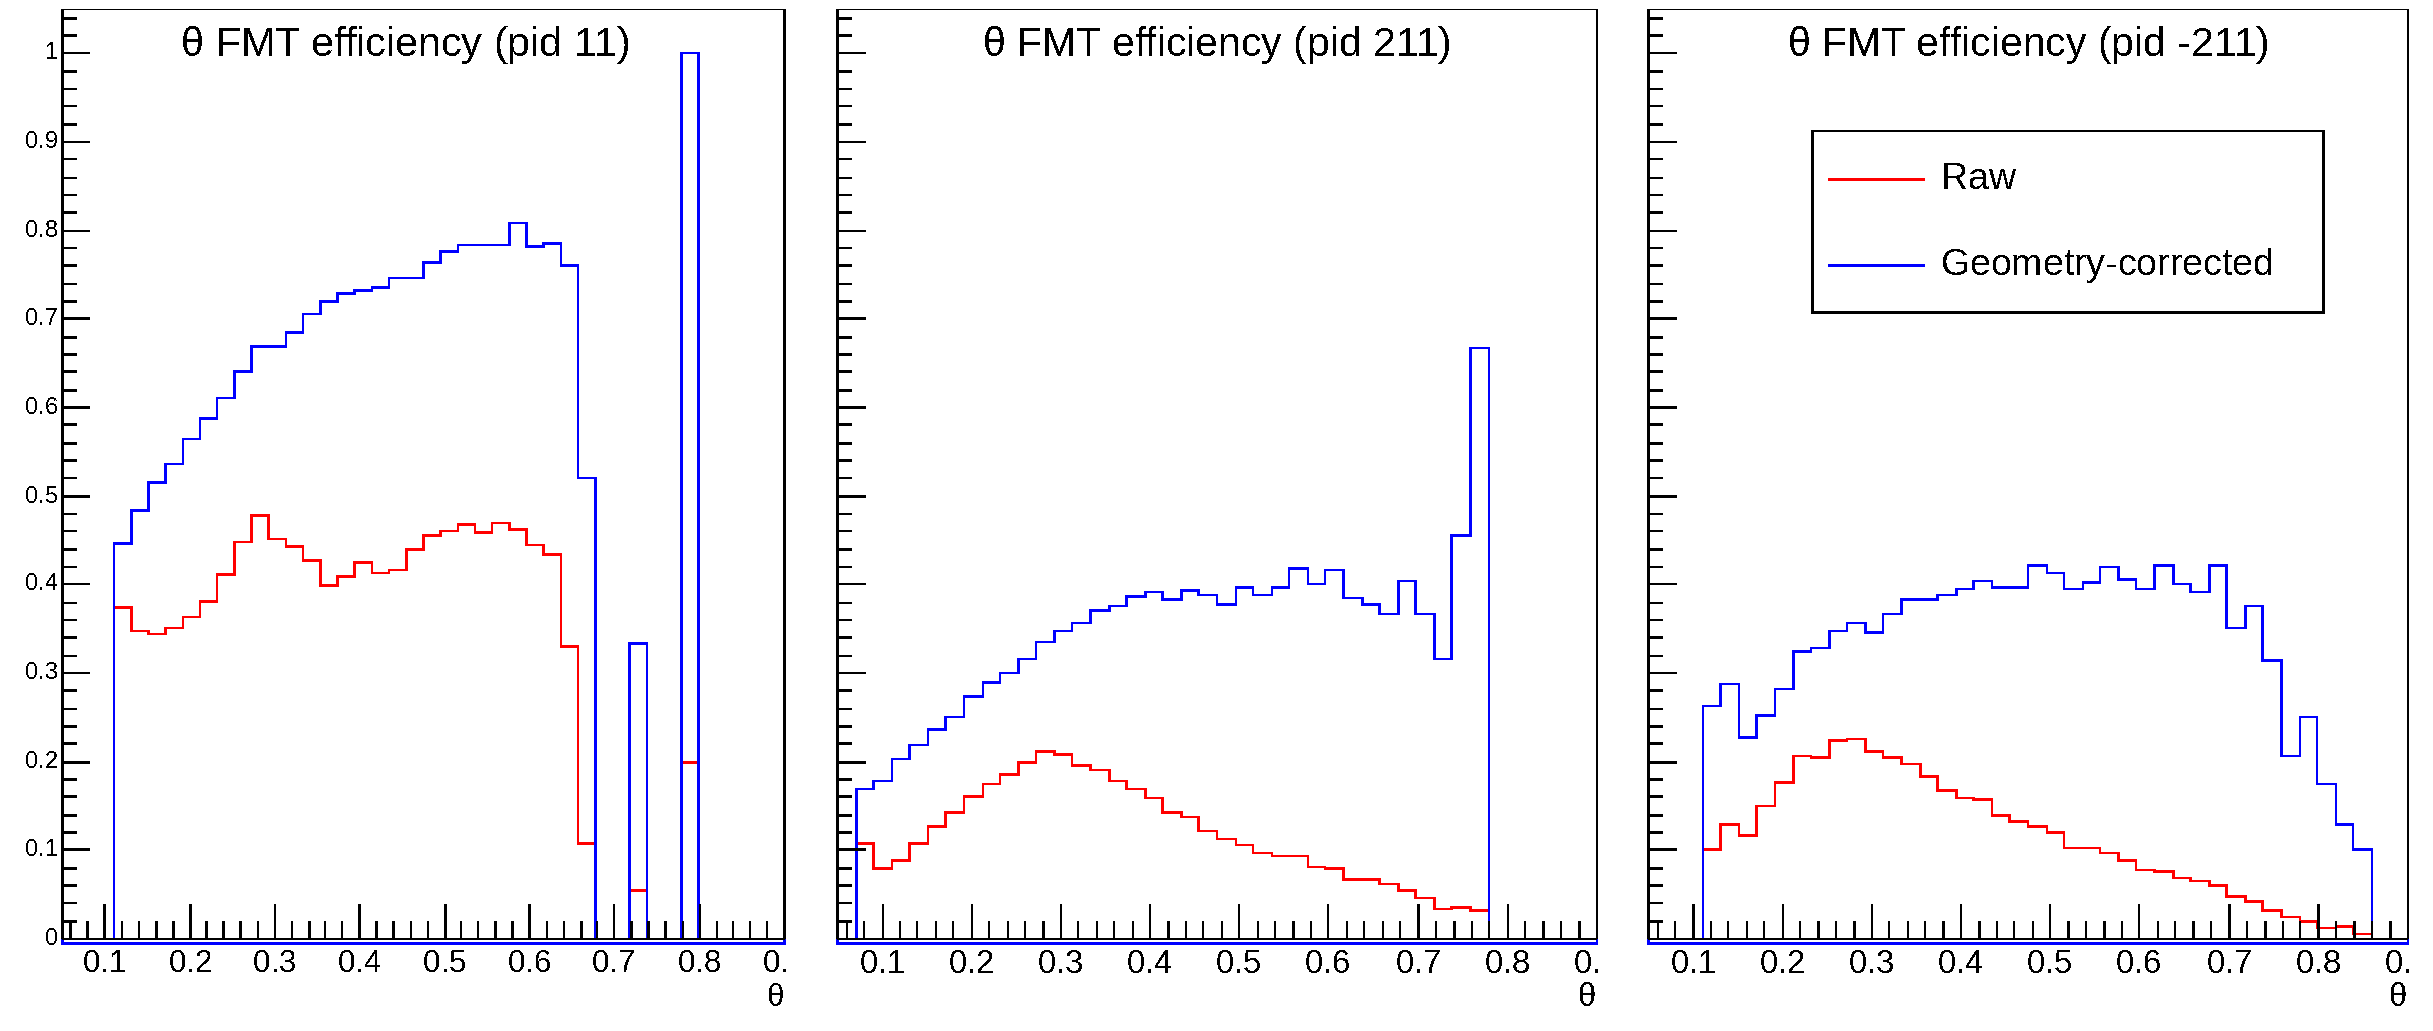
\includegraphics[width=\textwidth]{14theta_efficiency.pdf}
            \caption{$\theta$ FMT efficiency.}
            \label{fig::14.14::fmt_efficiency_theta}
        \end{subfigure}
        % p.
        \begin{subfigure}[b]{\textwidth}
            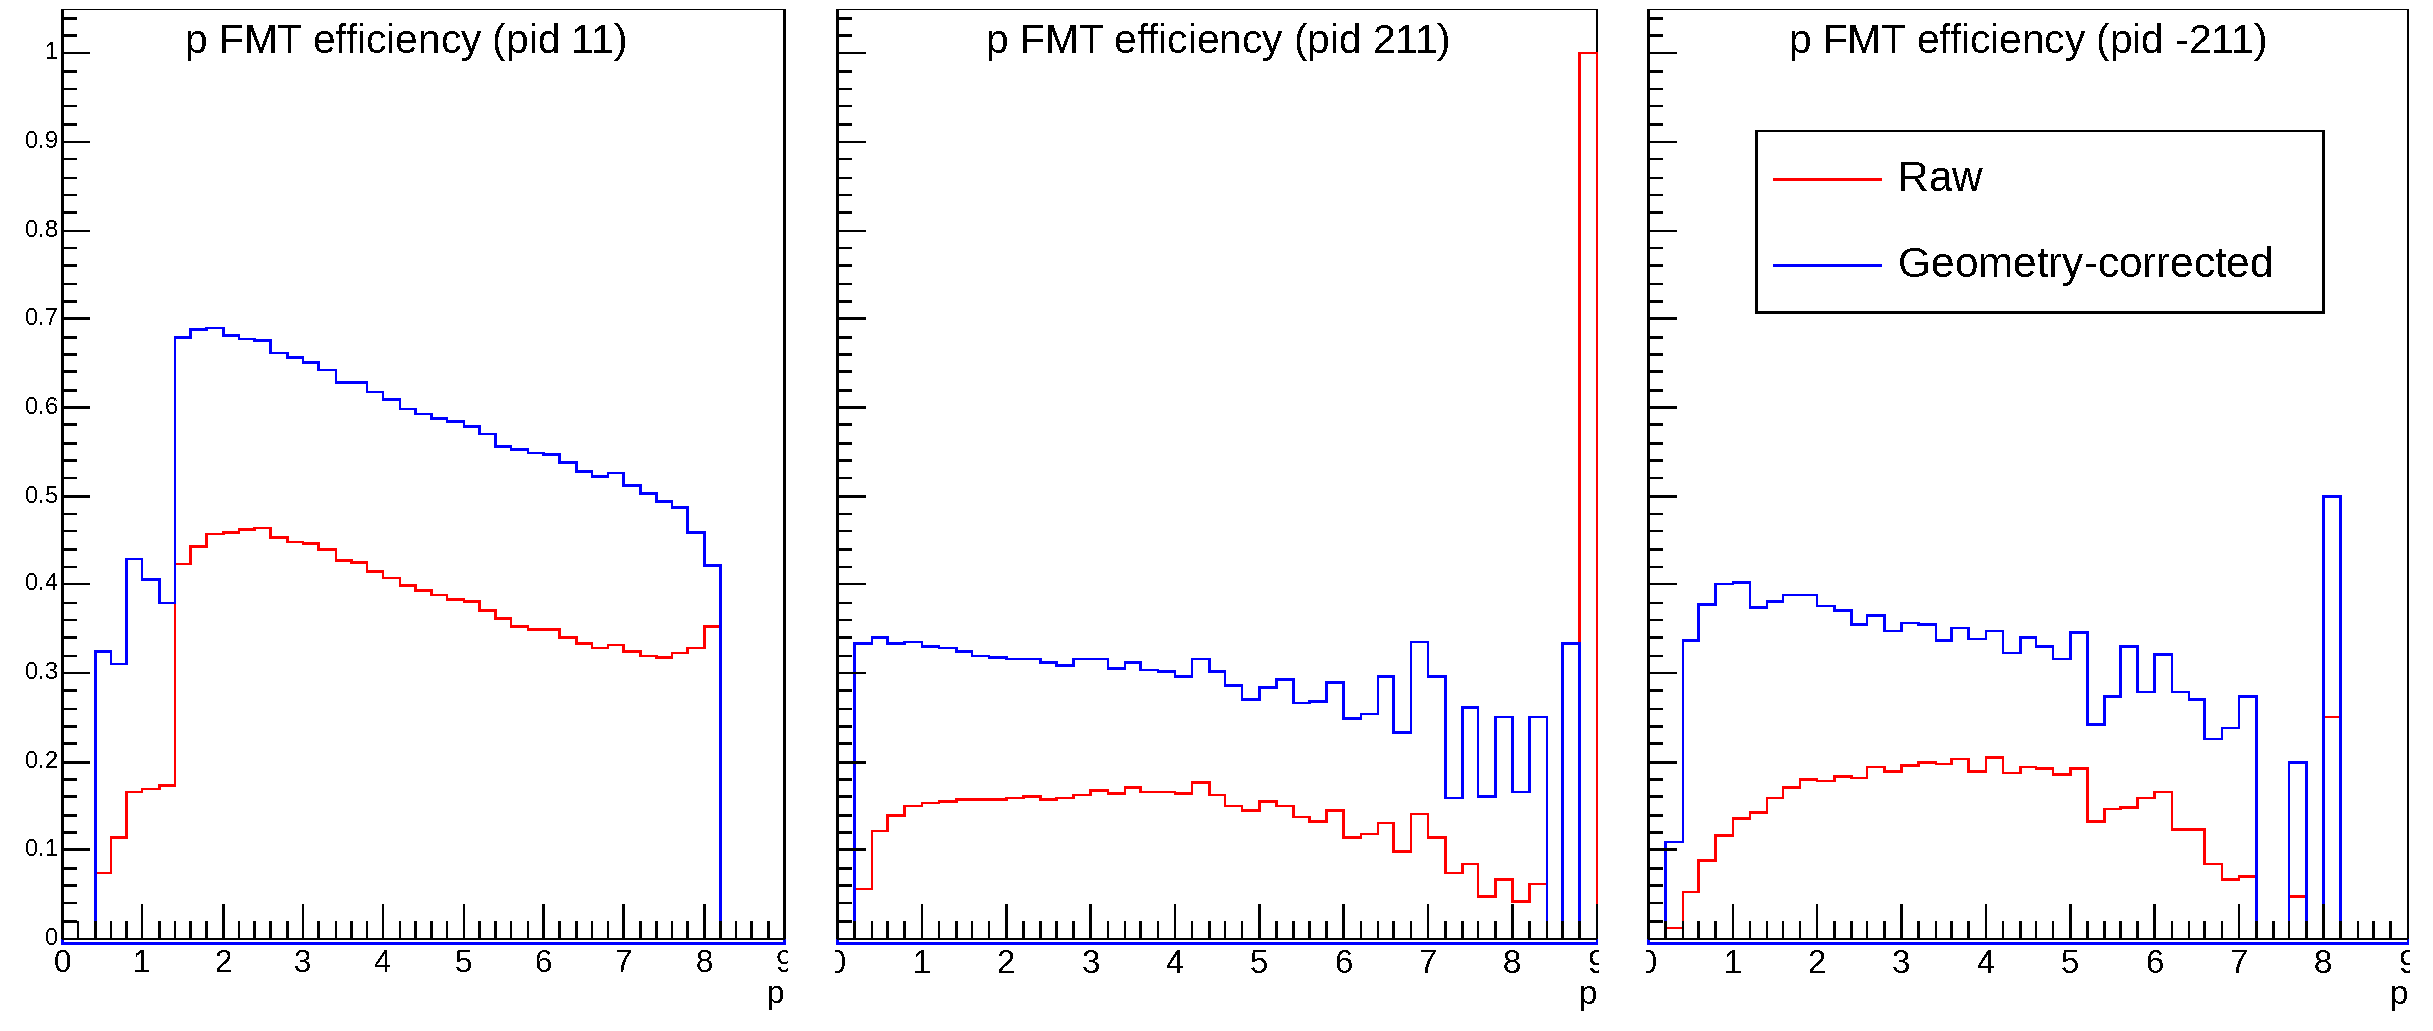
\includegraphics[width=\textwidth]{14p_efficiency.pdf}
            \caption{$p$ FMT efficiency.}
            \label{fig::14.14::fmt_efficiency_p}
        \end{subfigure}

        \caption[$v_z$, $\theta$, and $p$ FMT efficiencies for $e^-$, $e^-\pi^+$, and $e^-\pi^-$]
        {$v_z$, $\theta$, and $p$ FMT efficiencies for $e^-$, $e^-\pi^+$, and $e^-\pi^-$.
        FMT efficiency is defined as the percentage of DC tracks that are detected by 2 FMT layers.
        Run 12016.}
        \floatfoot{Source: Own elaboration, using the \href{https://github.com/bleaktwig/clas12-rge-analysis}{clas12-rge-analysis} software.}
        \label{fig::14.14::fmt_efficiencies}
    \end{figure}

    \begin{figure}
        % phi efficiency.
        \begin{subfigure}[b]{\textwidth}
            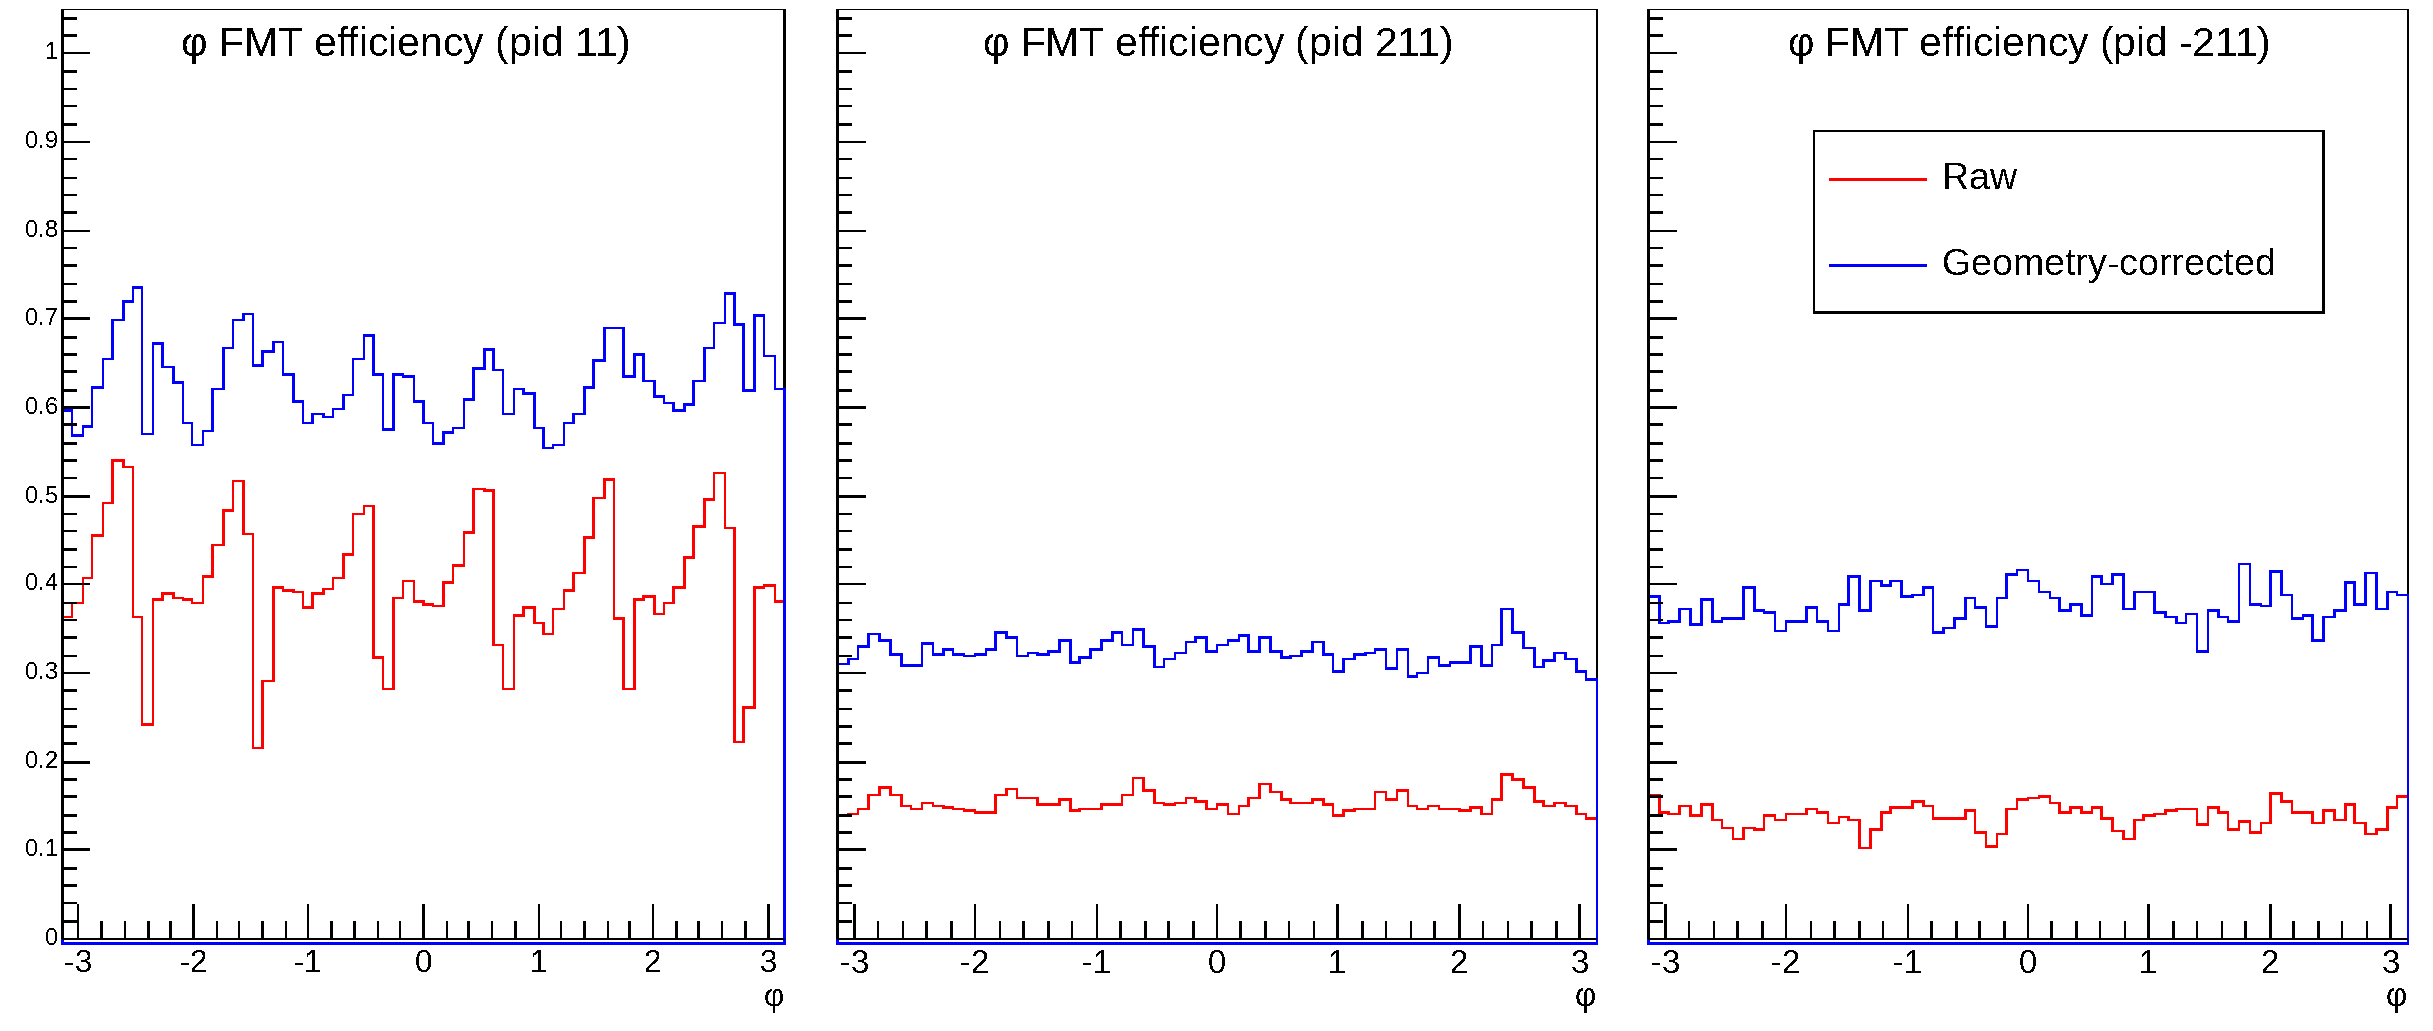
\includegraphics[width=\textwidth]{14phi_efficiency.pdf}
            \caption{$\phi$ FMT efficiency for $e^-$, $e^-\pi^+$, and $e^-\pi^-$.
            FMT efficiency is defined as the percentage of DC tracks that are detected by 2 FMT layers.}
            \label{fig::14.14::fmt_efficiency_phi}
        \end{subfigure}
        % geometry cut effect.
        \begin{subfigure}[b]{\textwidth}
            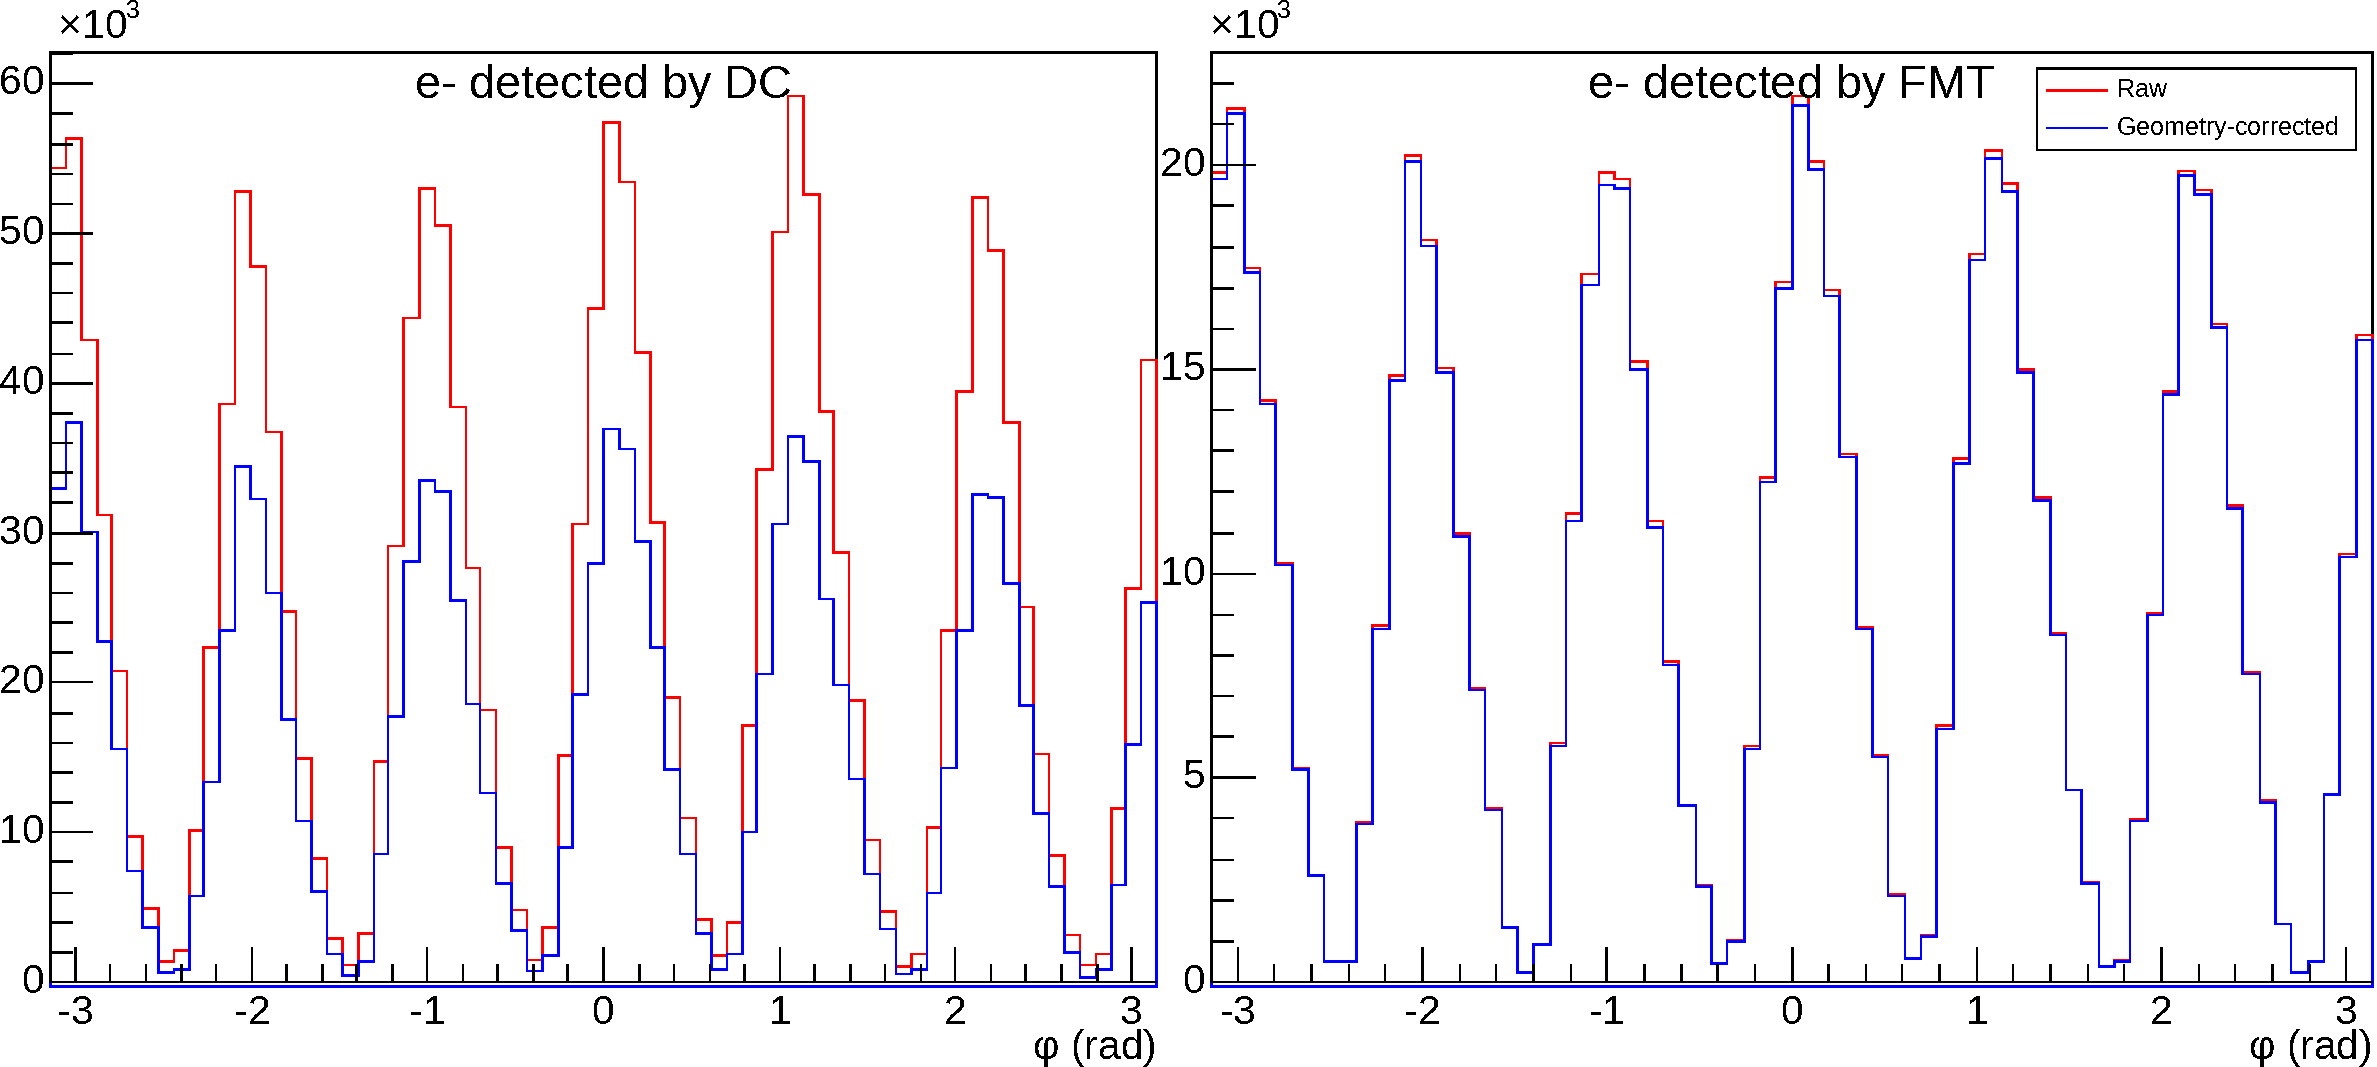
\includegraphics[width=\textwidth]{14phi_geomcut.pdf}
            \caption{Number of electrons detected in terms of $\phi$ for DC and FMT.}
            \label{fig::14.14::phi_geomcut}
        \end{subfigure}

        \caption[$\phi$ efficiency and geometry cut study]
        {$\phi$ FMT efficiency and number of $e^-$ detected for DC and FMT.
        Run 12016.}
        \floatfoot{Source: Own elaboration, using the \href{https://github.com/bleaktwig/clas12-rge-analysis}{clas12-rge-analysis} software.}
        \label{fig::14.14::phi_study}
    \end{figure}

    Our prediction is validated by Figures \ref{fig::14.14::fmt_efficiency_vz} and \ref{fig::14.14::fmt_efficiency_theta}.
    The efficiency displays a pronounced dependence on both $v_z$ and $\theta$ for all three particles under study.
    It is worth noting that the dependence is more pronounced for electrons compared to pions.
    This outcome aligns with expectations, as the only accepted pions are those detected in events where an electron is also detected.
    Thus, the ``final'' pion efficiency incorporates the combined detector efficiencies for electrons and pions.

    Next, Figure \ref{fig::14.14::fmt_efficiency_p} confirms our expectation that there is no strong correlation between efficiency and momentum.

    Last, we examine the $\phi$ efficiency, as depicted in Figure \ref{fig::14.14::fmt_efficiency_phi}.
    Our prediction holds true for both positive and negative pions, as the efficiency demonstrates no dependence on the value of $\phi$.
    However, in the case of electrons, upon initial inspection, the sharp valleys appear less prominent after applying the geometry cut.

    Nevertheless, this is merely a visual effect.
    When we tally the number of electrons detected by the DC and FMT, the valleys become more pronounced in the DC, while they remain the same in the FMT.
    Consequently, the increase in FMT efficiency becomes more pronounced in these valleys, as demonstrated in Figure \ref{fig::14.14::phi_geomcut}.

    As can be seen in Table \ref{tab::14.14::fmt_efficiency_study} and Figures \ref{fig::14.14::fmt_efficiencies} and \ref{fig::14.14::phi_study}, the pion efficiency for 3-layer tracks does not exceed $3\%$.
    Consequently, it is not practical to work exclusively with FMT tracks that traverse all three FMT layers in this study.
    For the remainder of the document, 2 and 3-layer tracks will be considered together, and will be collectively referred to as FMT tracks.


    % !TEX root = ../main.tex
\subsection{Acceptance Correction Results}
\label{14.20::acceptance_correction_results}
    % !TEX root = ../main.tex
\subsubsection{Electron Variables}
\label{14.21::electron_variables}
    The acceptance of the scattered electron variables $Q^2$ and $\nu$ is presented in Figure \ref{fig::14.21::electron_acc}.
    Each one is shown in an integrated kinematical region for the other variable.

    \begin{figure}[t!]
        \centering
        % Q2.
        \begin{subfigure}[b]{\textwidth}
            \centering
            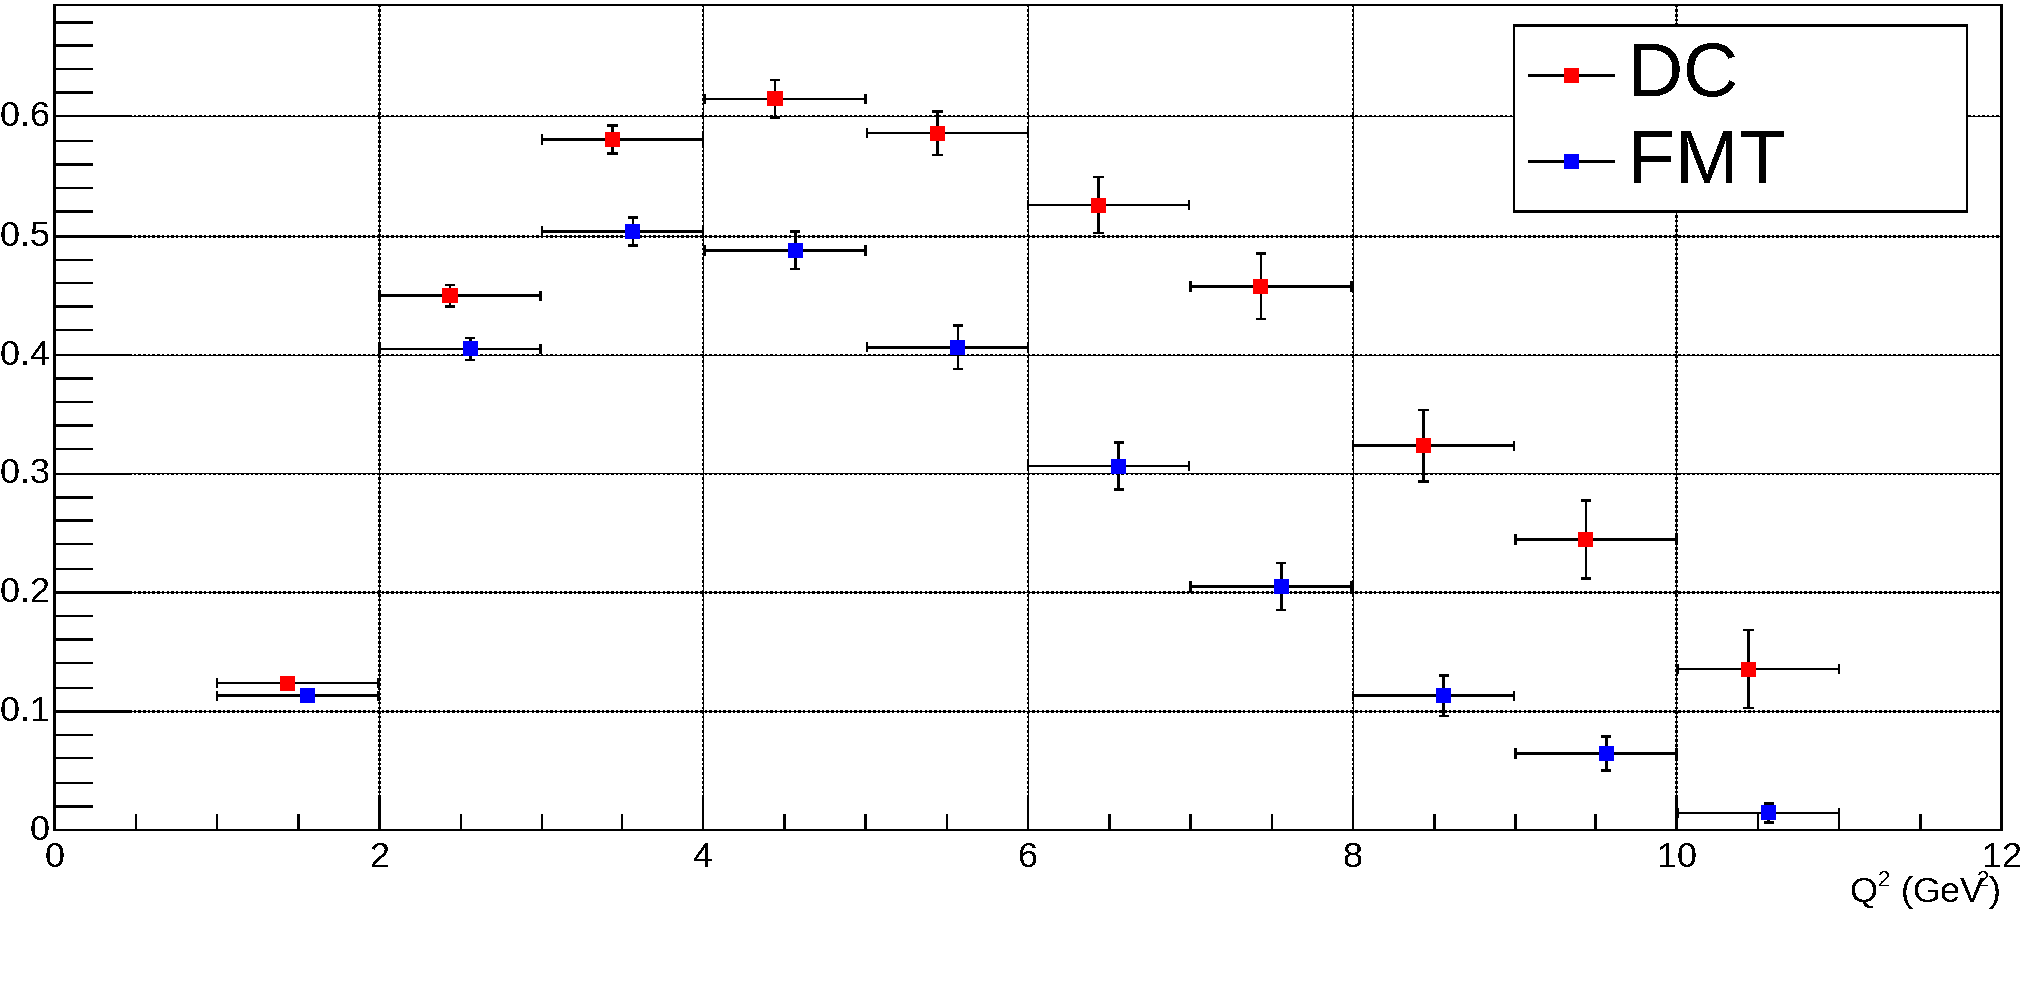
\includegraphics[width=\textwidth]{21q2_acc.pdf}
            \caption{$Q^2$ acceptance.}
            \label{fig::14.21::q2_acc}
        \end{subfigure}
        \hfill
        % nu.
        \begin{subfigure}[b]{\textwidth}
            \centering
            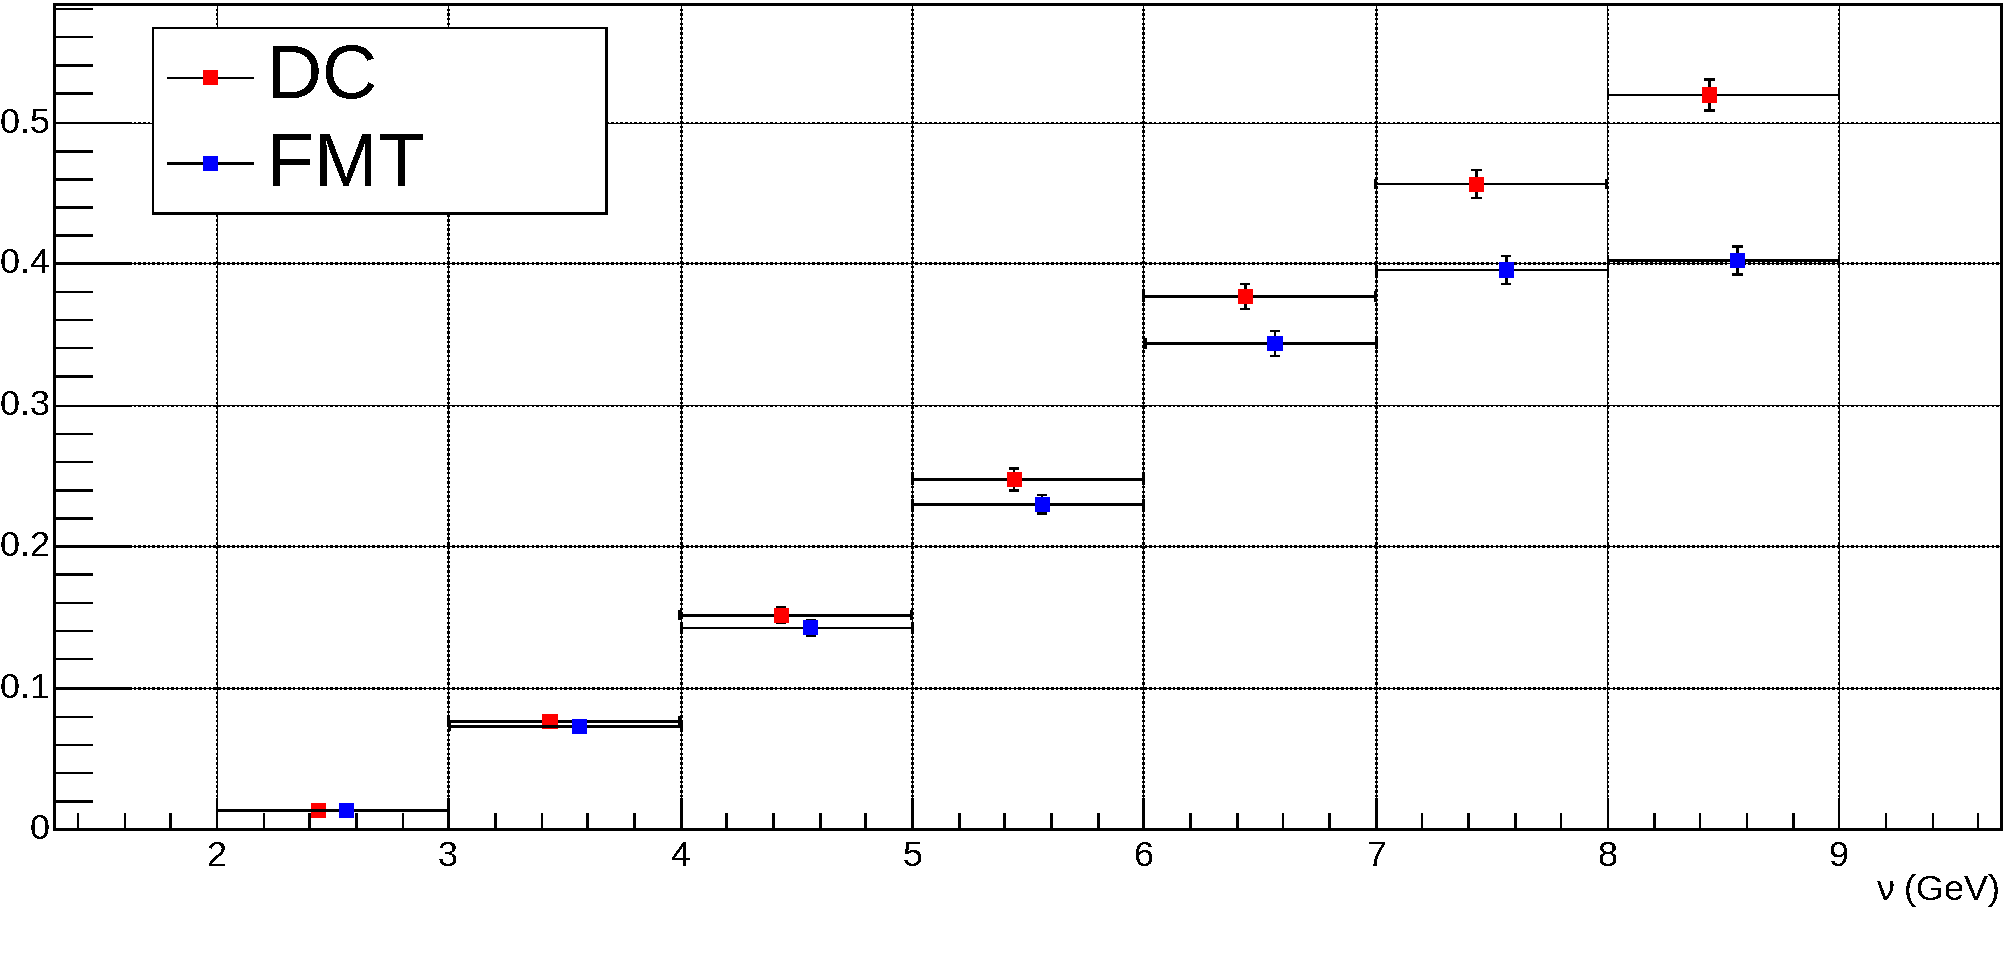
\includegraphics[width=\textwidth]{21nu_acc.pdf}
            \caption{$\nu$ acceptance.}
            \label{fig::14.21::nu_acc}
        \end{subfigure}
        \caption[$e^-$ variables acceptance]
        {$e^-$ variables acceptance.
        $\nu$ is integrated in \ref{fig::14.21::q2_acc}, and $Q^2$ is integrated in \ref{fig::14.21::nu_acc}.
        The bin markers are slightly shifted in $x$ to improve legibility.}
        \floatfoot{Source: Own elaboration, using the \href{https://github.com/bleaktwig/clas12-rge-analysis}{clas12-rge-analysis} software.}
        \label{fig::14.21::electron_acc}
    \end{figure}

    \begin{figure}
        \centering
        % phi vs. theta.
        \begin{subfigure}[b]{\textwidth}
            \centering
            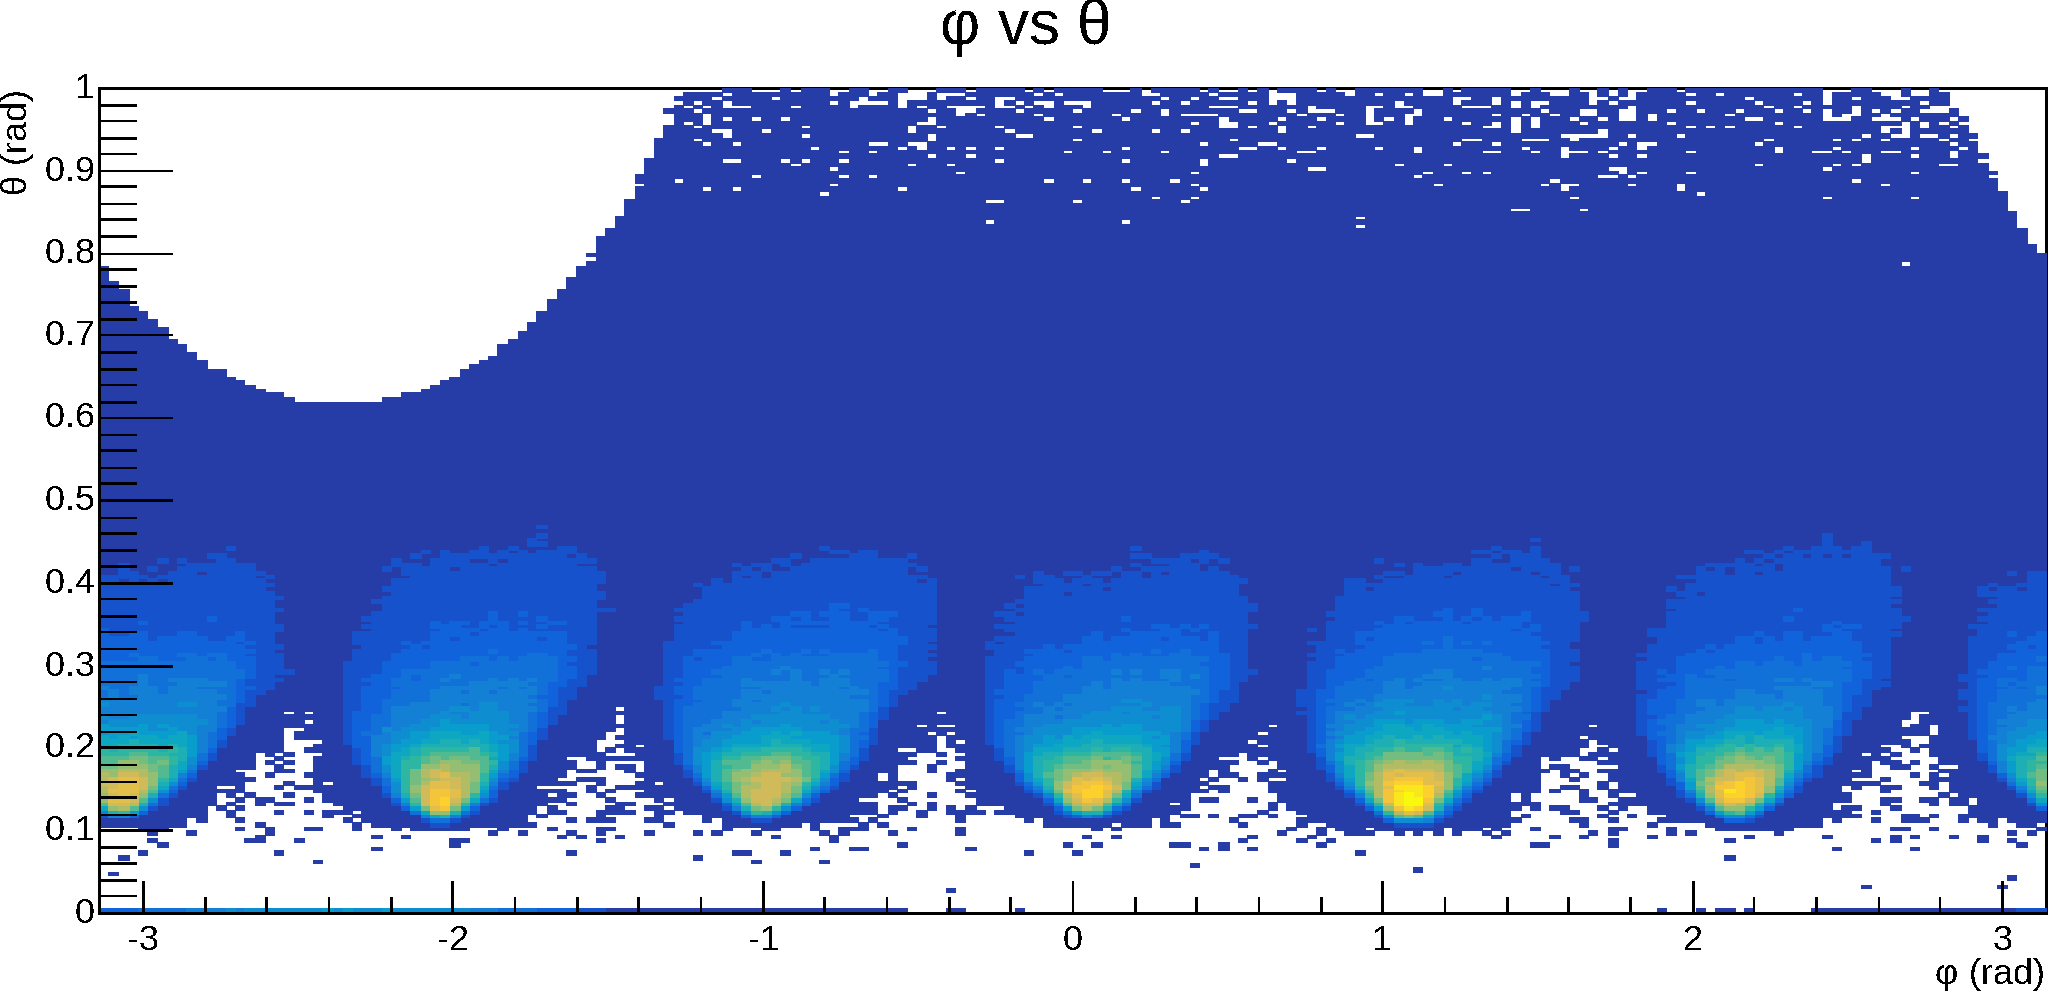
\includegraphics[width=\textwidth]{21phi_theta_neg.pdf}
            \caption[$\phi$ vs. $\theta$ for negative particles]
            {$\phi$ vs. $\theta$ for negative particles detected by DC.}
            \label{fig::14.21::phi_theta_neg}
        \end{subfigure}
        % theta.
        \begin{subfigure}[b]{\textwidth}
            \centering
            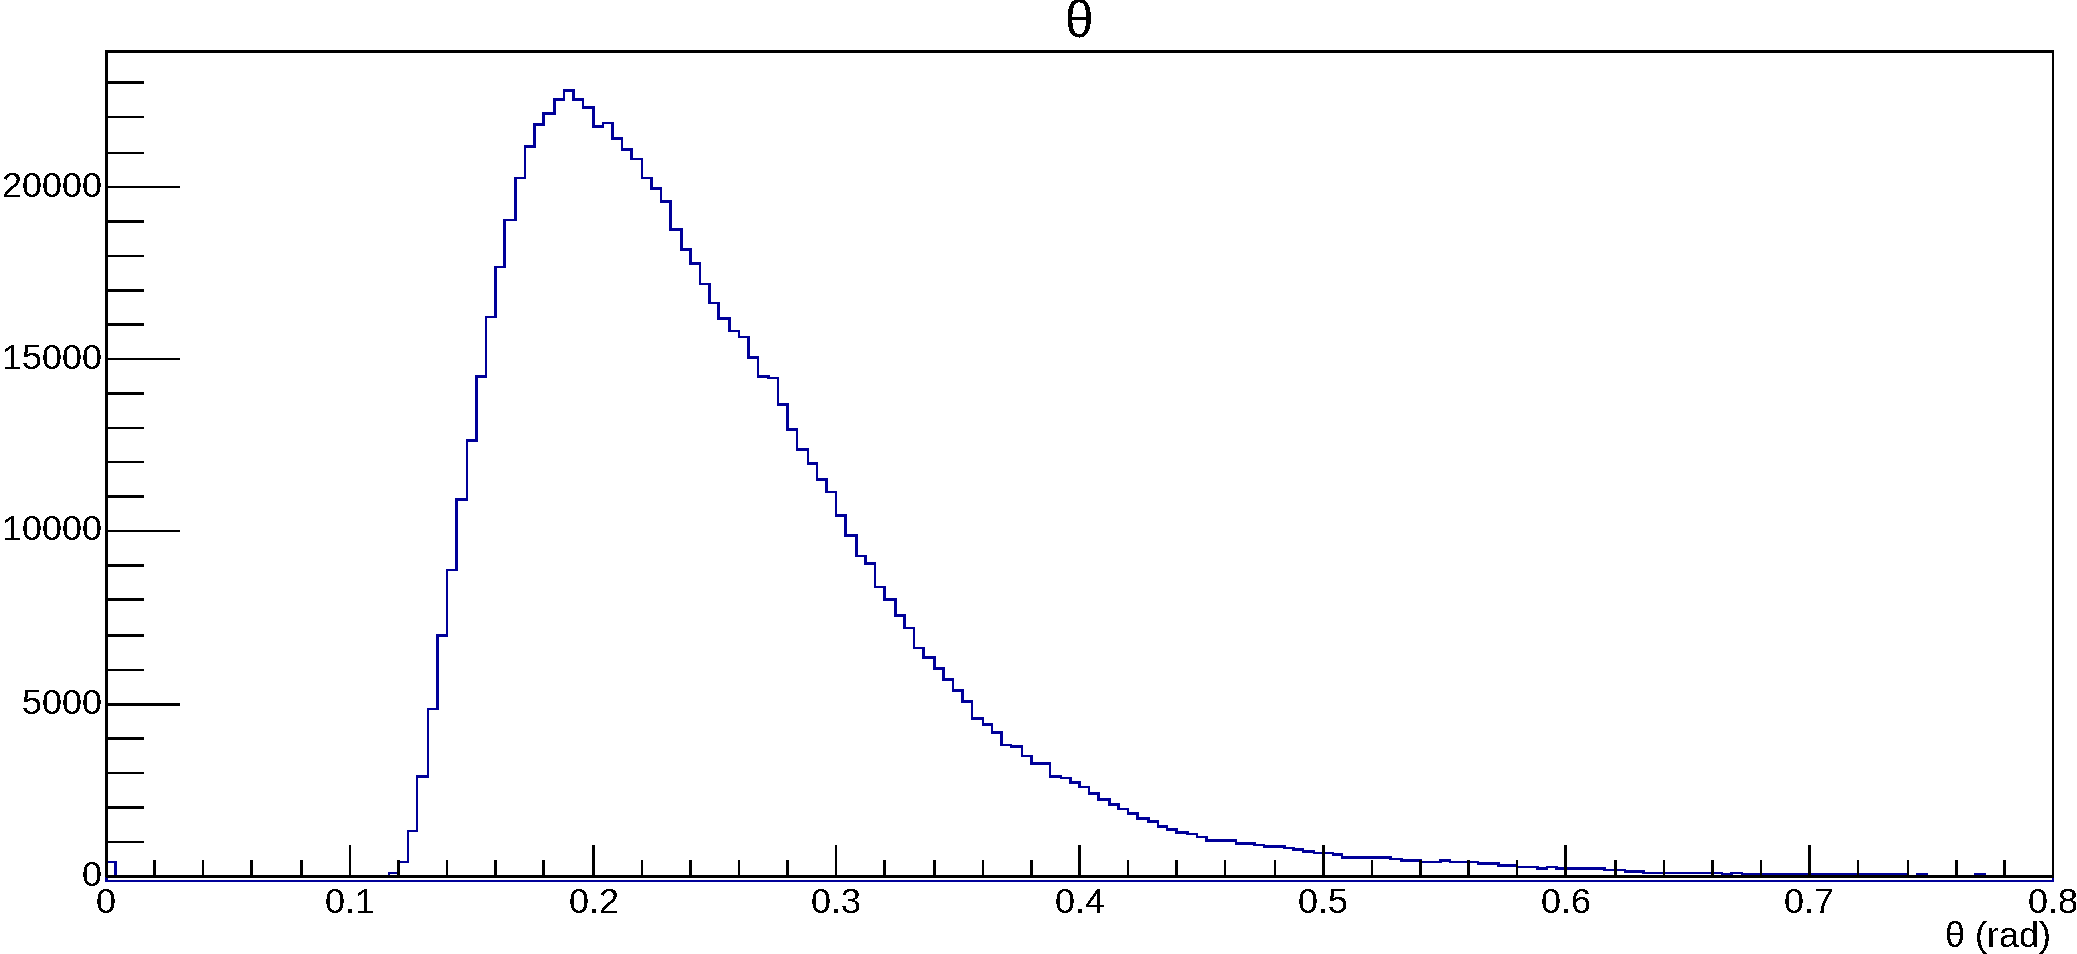
\includegraphics[width=\textwidth]{21theta_neg.pdf}
            \caption[$\theta$ for negative particles]
            {$\theta$ for negative particles detected by DC.}
            \label{fig::14.21::theta_neg}
        \end{subfigure}
        \caption[$\theta$ study for negative particles]
        {$\theta$ study for negative particles.
        Simulated RG-F target.}
        \floatfoot{Source: Own elaboration, using the \href{https://github.com/bleaktwig/clas12-rge-analysis}{clas12-rge-analysis} software.}
        \label{fig::14.21::theta_study_neg}
    \end{figure}

    % Q2.
    In Equation \eqref{eq::13.23::q2}, it can be observed that $Q^2$ has a quadratic dependence on the scattering angle $\theta_C$ of the scattered electrons.%, particularly for small angles.
    Hence, it is important to understand the $\theta$ acceptance of CLAS12 in order to distinguish the geometric effect related to $\theta$ from the inherent $Q^2$ acceptance of the FD.
    Figure \ref{fig::14.21::theta_study_neg} illustrates this dependence for negative particles.

    The triangular shape of each DC sector, combined with the inbending tracks resulting from the negative torus field, leads to a significantly low acceptance at low $\theta$ angles.
    When integrating across $\phi$, this results in a low $\theta$ efficiency for $\theta \lsim 0.15$ radians.
    Referring back to the $Q^2$ plot in Figure \ref{fig::14.21::q2_acc}, the decrease in $Q^2$ acceptance between 1 and 4 $GeV^2$ can be clearly attributed to this geometric effect, which is purely of a geometric nature.

    % nu
    On the other hand, since $\nu$ does not exhibit a direct correlation with $\theta_C$ (as indicated by Equation \eqref{eq::13.23::nu}), we can assume that the acceptance observed in Figure \ref{fig::14.21::nu_acc} is intrinsic to the detector.

    % !TEX root = ../main.tex
\subsubsection{Hadronic Variables}
\label{14.22::hadronic_variables}
    Next, we'll look at $z_h$, $p_T^2$, and $\phi_{PQ}$ acceptances for $e^-\pi^+$ and $e^-\pi^-$.
    It's worth noting that these acceptances are lower than those for electron variables.
    This is to be expected, since they require both the trigger electron and at least one hadron to be accepted by the detector, as is seen also on their efficiencies, as presented in Table \ref{tab::14.14::fmt_efficiency_study}

    \textbf{TODO. Say something?}

    We can see $z_h$ acceptance in Figure \textbf{TODO}, where... (TODO).

    Next, $p_T^2$ acceptance is presented in Figure \textbf{TODO}, where we see that... (TODO).

    Finally, $\phi_{PQ}$ acceptance is studied in Figure \textbf{TODO}.
    Here, we see... (TODO).

    % zh.
    \begin{figure}
        \centering
        % pi+.
        \begin{subfigure}[b]{0.49\textwidth}
            \centering
            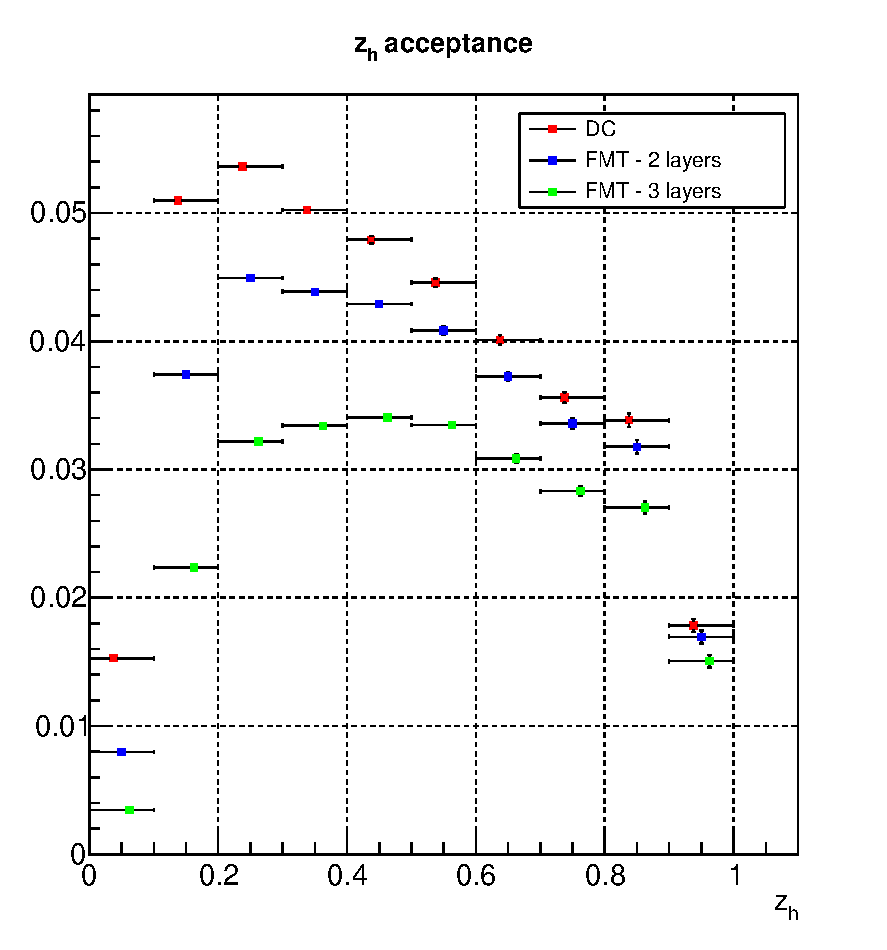
\includegraphics[width=\textwidth]{22zh_acc_211.pdf}
            \caption{$z_h$ acceptance for $e^-\pi^+$.}
            \label{fig::14.22::zh_acc_211}
        \end{subfigure}
        \hfill
        % pi-.
        \begin{subfigure}[b]{0.49\textwidth}
            \centering
            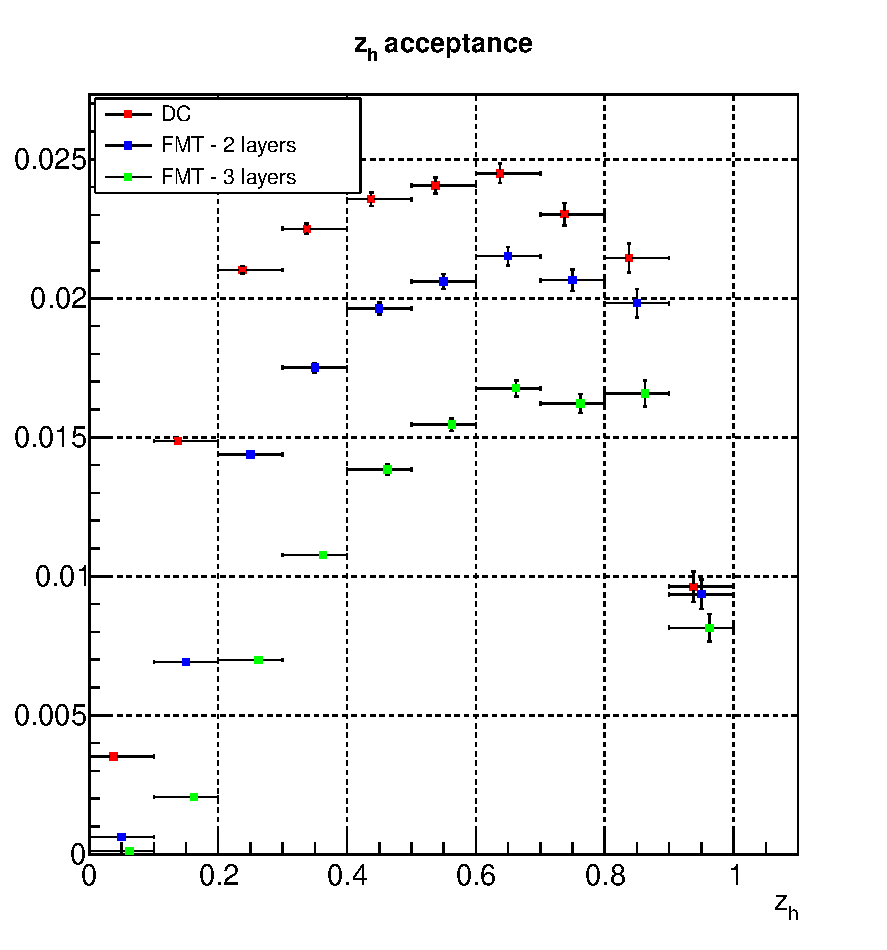
\includegraphics[width=\textwidth]{22zh_acc_-211.pdf}
            \caption{$z_h$ acceptance for $e^-\pi^-$.}
            \label{fig::14.22::zh_acc_-211}
        \end{subfigure}
        \caption[$z_h$ acceptance.]{$z_h$ acceptance for $e^-\pi^+$ and $e^-\pi^-$.
        All electron and other hadronic variables are integrated in both plots.
        The bin markers are slightly shifted in $x$ to improve legibility.
        Source: Own elaboration, using the \href{https://github.com/bleaktwig/clas12-rge-analysis}{clas12-rge-analysis} software.}
        \label{fig::14.22::zh_acc}
    \end{figure}

    % Pt2.
    \begin{figure}
        \centering
        % pi+.
        \begin{subfigure}[b]{0.49\textwidth}
            \centering
            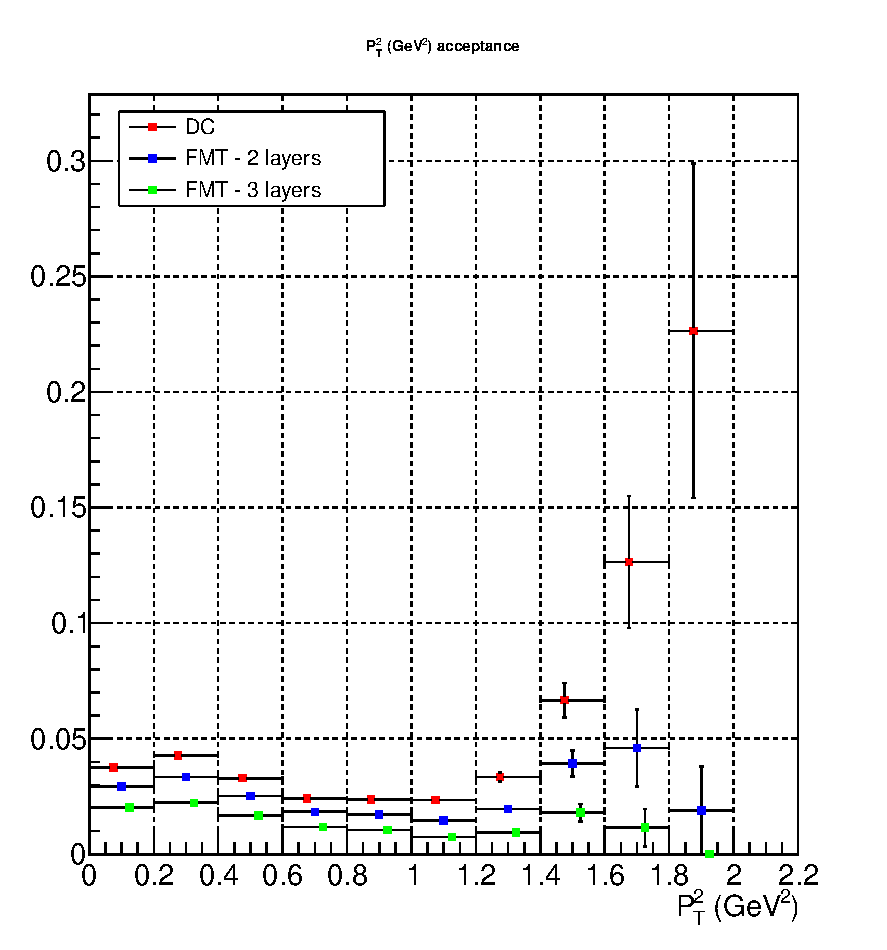
\includegraphics[width=\textwidth]{22pt2_acc_211.pdf}
            \caption{$p_T^2$ acceptance for $e^-\pi^+$.}
            \label{fig::14.22::pt2_acc_211}
        \end{subfigure}
        \hfill
        % pi-.
        \begin{subfigure}[b]{0.49\textwidth}
            \centering
            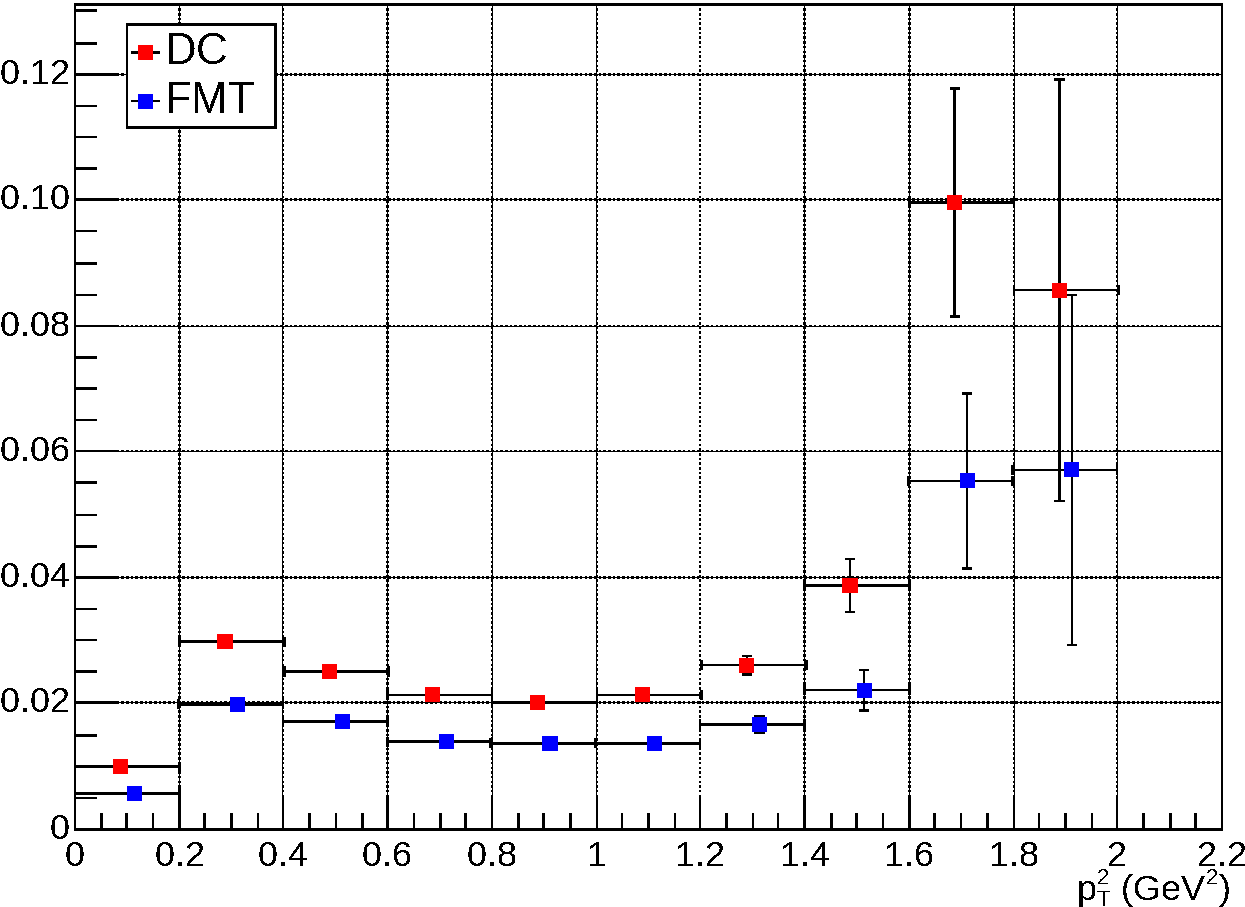
\includegraphics[width=\textwidth]{22pt2_acc_-211.pdf}
            \caption{$p_T^2$ acceptance for $e^-\pi^-$.}
            \label{fig::14.22::pt2_acc_-211}
        \end{subfigure}
        \caption[$p_T^2$ acceptance.]{$p_T^2$ acceptance for $e^-\pi^+$ and $e^-\pi^-$.
        All electron and other hadronic variables are integrated in both plots.
        The bin markers are slightly shifted in $x$ to improve legibility.
        Source: Own elaboration, using the \href{https://github.com/bleaktwig/clas12-rge-analysis}{clas12-rge-analysis} software.}
        \label{fig::14.22::pt2_acc}
    \end{figure}

    % phipq.
    \begin{figure}
        \centering
        % pi+.
        \begin{subfigure}[b]{0.49\textwidth}
            \centering
            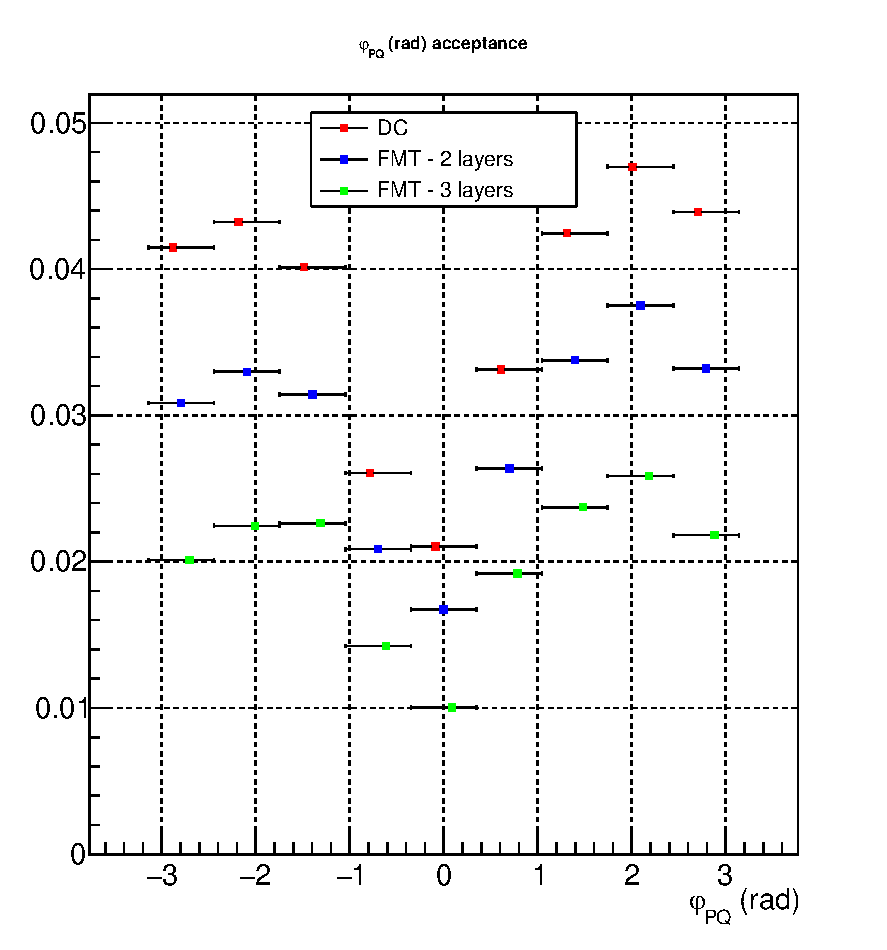
\includegraphics[width=\textwidth]{22phipq_acc_211.pdf}
            \caption{$\phi_{PQ}$ acceptance for $e^-\pi^+$.}
            \label{fig::14.22::phipq_acc_211}
        \end{subfigure}
        \hfill
        % pi-.
        \begin{subfigure}[b]{0.49\textwidth}
            \centering
            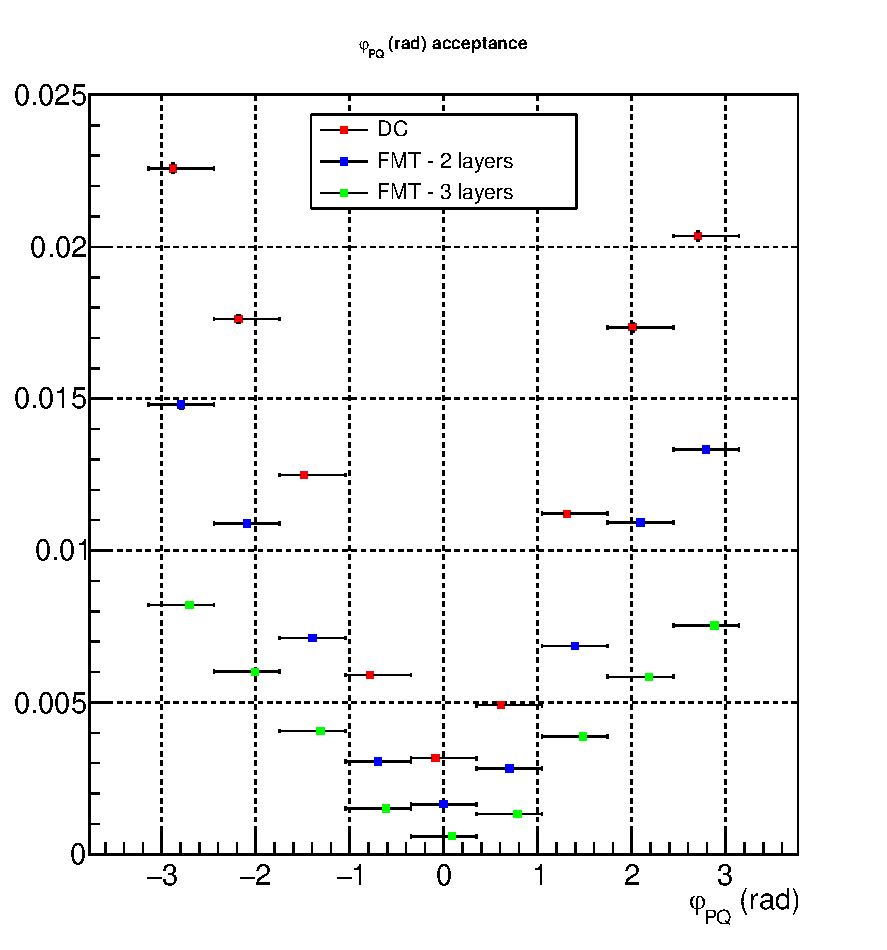
\includegraphics[width=\textwidth]{22phipq_acc_-211.pdf}
            \caption{$\phi_{PQ}$ acceptance for $e^-\pi^-$.}
            \label{fig::14.22::phipq_acc_-211}
        \end{subfigure}
        \caption[$\phi_{PQ}$ acceptance.]{$\phi_{PQ}$ acceptance for $e^-\pi^+$ and $e^-\pi^-$.
        All electron and other hadronic variables are integrated in both plots.
        The bin markers are slightly shifted in $x$ to improve legibility.
        Source: Own elaboration, using the \href{https://github.com/bleaktwig/clas12-rge-analysis}{clas12-rge-analysis} software.}
        \label{fig::14.22::phipq_acc}
    \end{figure}


% --+ Plots +-------------------------------------------------------------------
    % \begin{figure}[hbtp]
    %     % Q2.
    %     \begin{subfigure}{.5\textwidth}
    %         \centering
    %         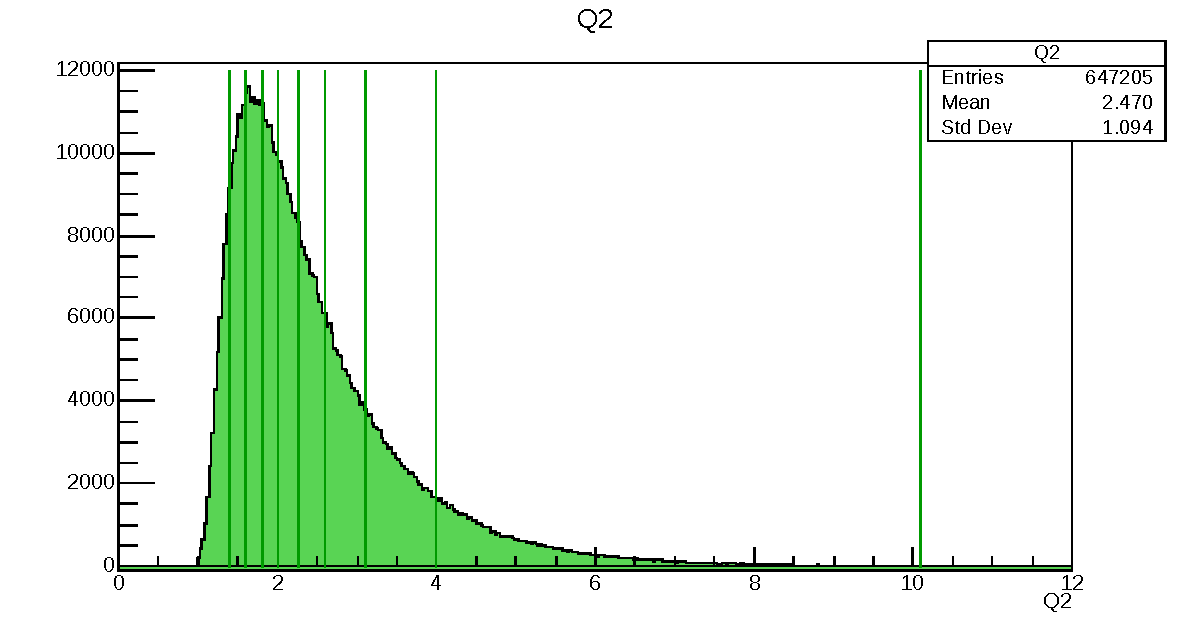
\includegraphics[width=\linewidth]{13dataanalysis/img/40_accbins_q2.pdf}
    %         % \caption{$Q^2$ bins.}
    %         \label{fig::acc_corr_bins_q2}
    %     \end{subfigure}
    %     \begin{subfigure}{.5\textwidth}
    %         \centering
    %         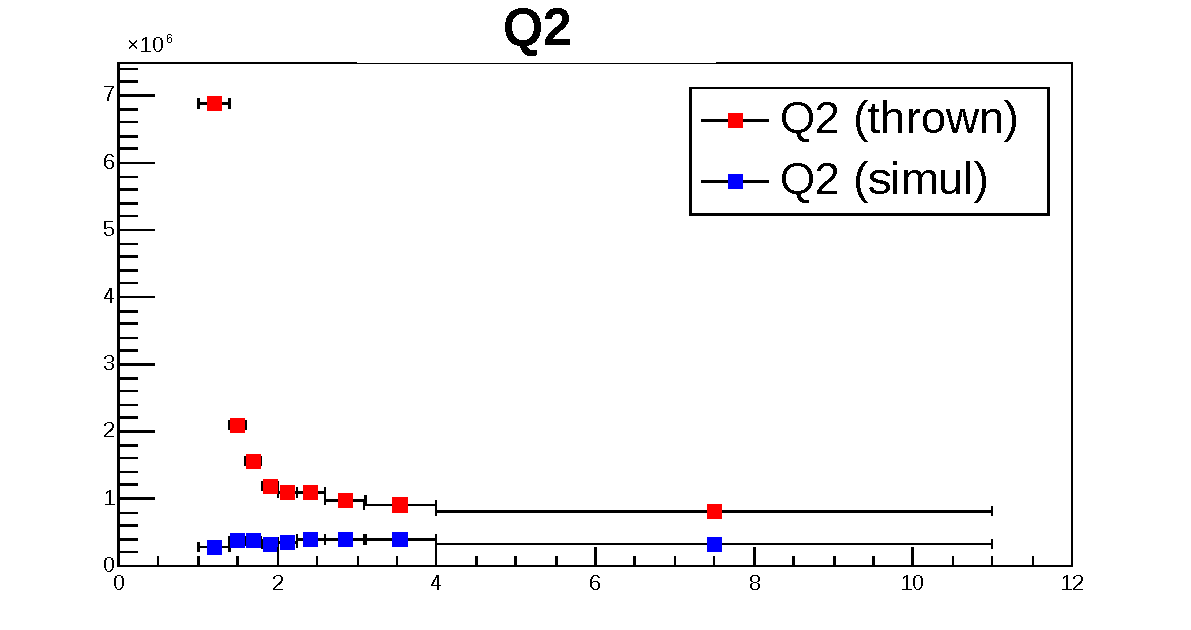
\includegraphics[width=\linewidth]{13dataanalysis/img/40_acccorr_q2.pdf}
    %         % \caption{$Q^2$ acceptance correction results.}
    %         \label{fig::acc_corr_q2}
    %     \end{subfigure}
    %
    %     % nu.
    %     \begin{subfigure}{.5\textwidth}
    %         \centering
    %         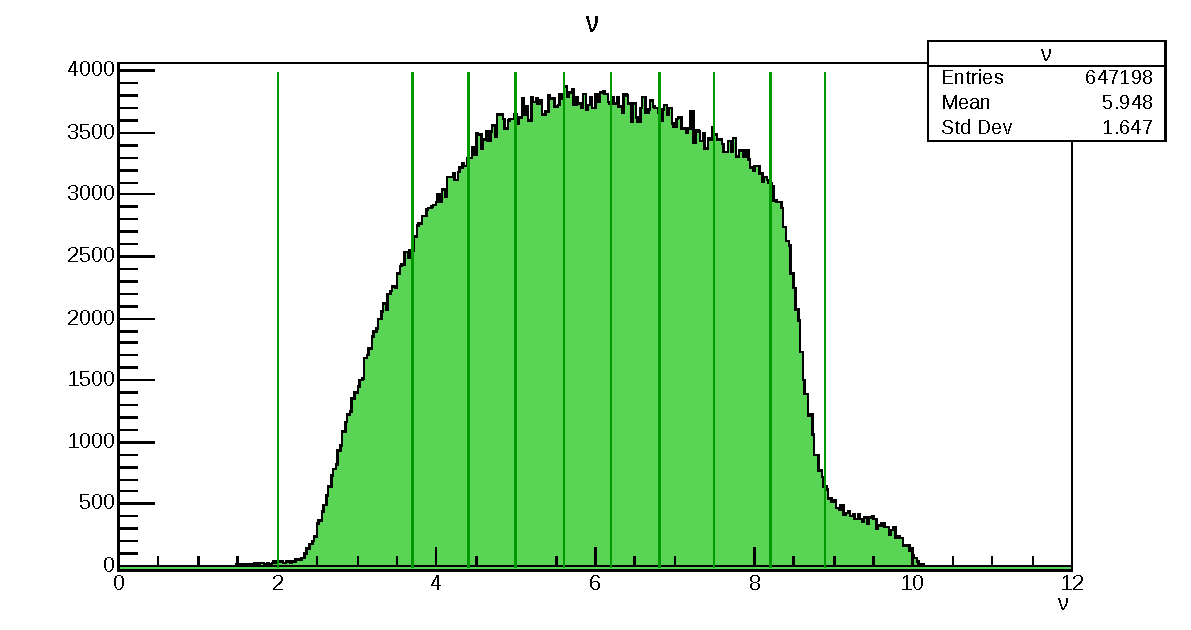
\includegraphics[width=\linewidth]{13dataanalysis/img/40_accbins_nu.pdf}
    %         % \caption{$\nu$ bins.}
    %         \label{fig::acc_corr_bins_nu}
    %     \end{subfigure}
    %     \begin{subfigure}{.5\textwidth}
    %         \centering
    %         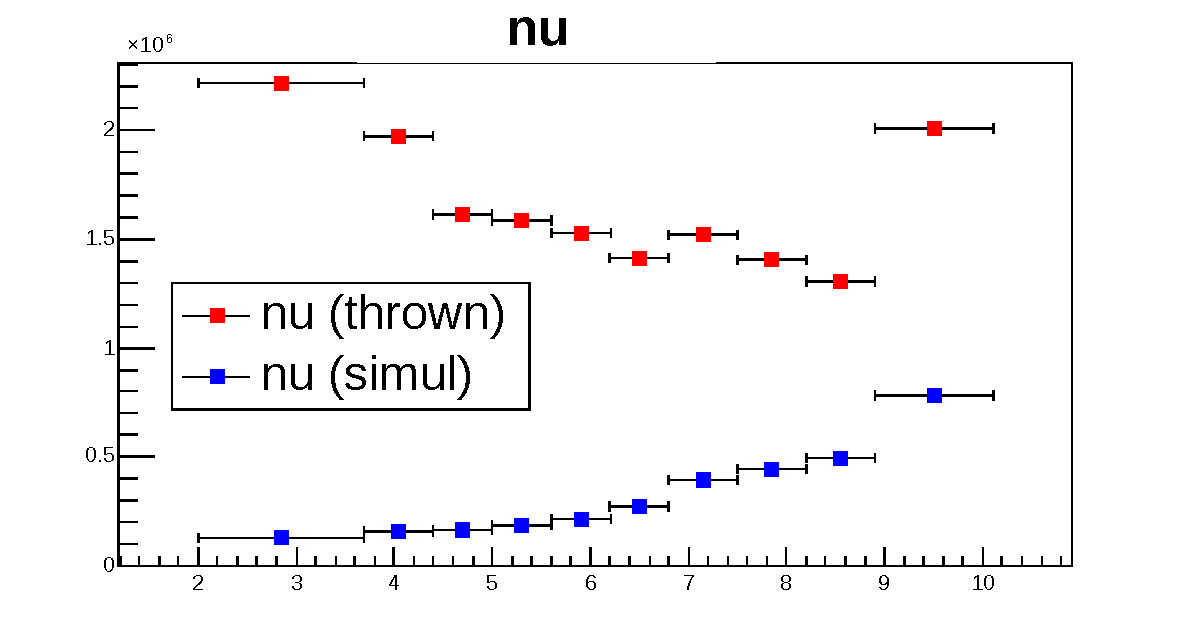
\includegraphics[width=\linewidth]{13dataanalysis/img/40_acccorr_nu.pdf}
    %         % \caption{$\nu$ acceptance correction results.}
    %         \label{fig::acc_corr_nu}
    %     \end{subfigure}
    %
    %     % zh.
    %     \begin{subfigure}{.5\textwidth}
    %         \centering
    %         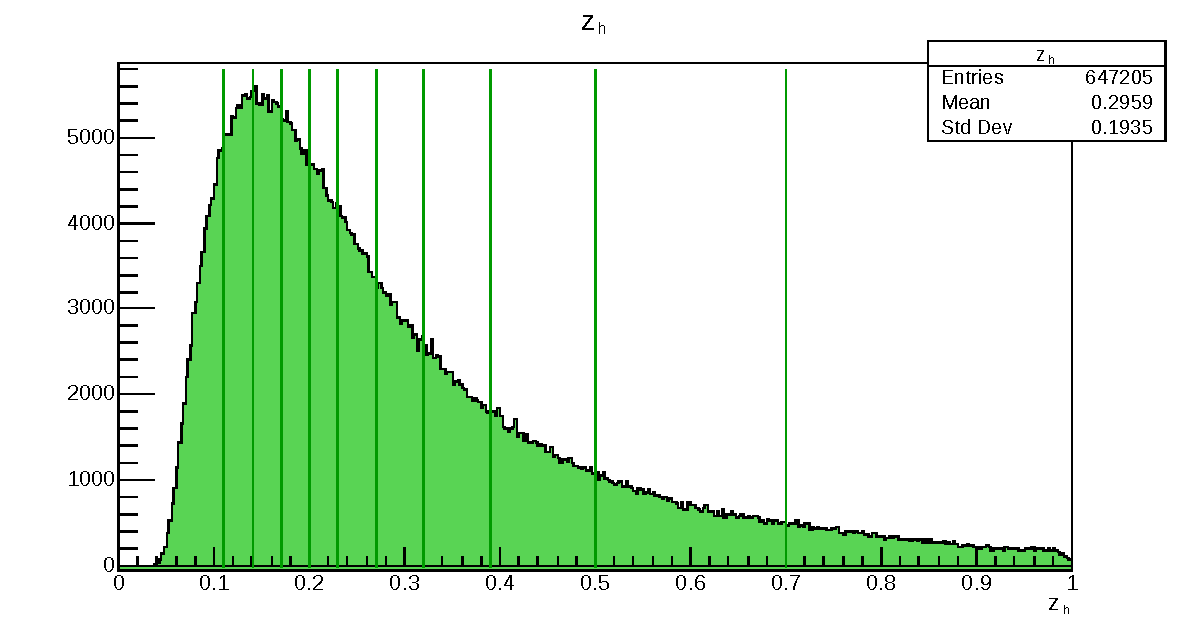
\includegraphics[width=\linewidth]{13dataanalysis/img/40_accbins_zh.pdf}
    %         % \caption{$z_h$ bins.}
    %         \label{fig::acc_corr_bins_zh}
    %     \end{subfigure}
    %     \begin{subfigure}{.5\textwidth}
    %         \centering
    %         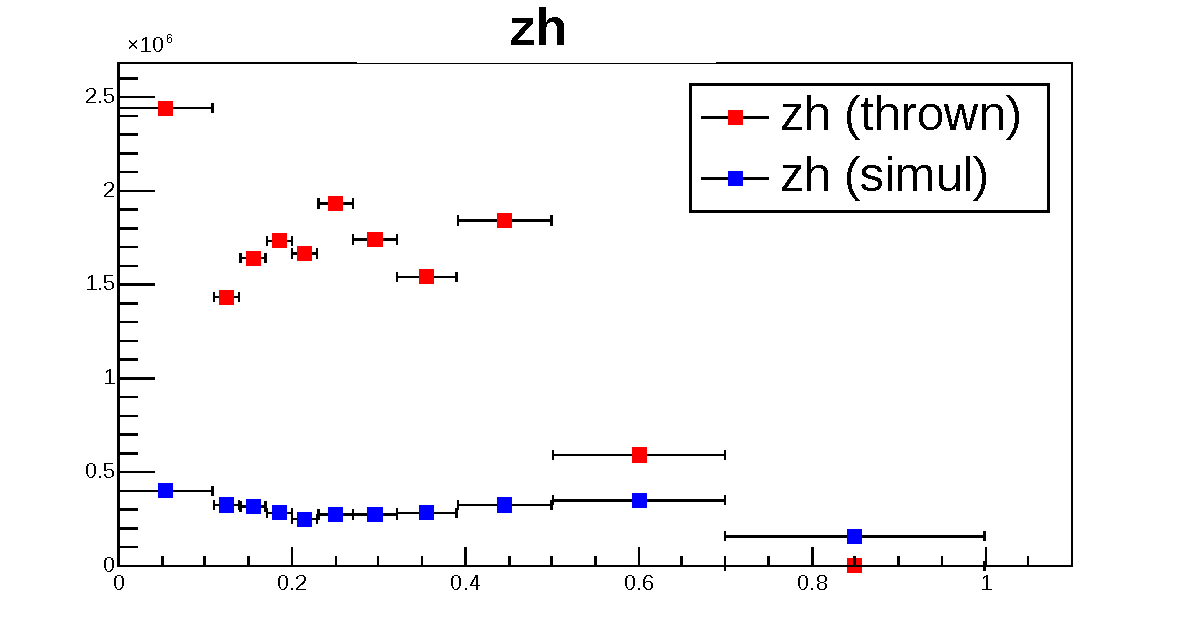
\includegraphics[width=\linewidth]{13dataanalysis/img/40_acccorr_zh.pdf}
    %         % \caption{$z_h$ acceptance correction results.}
    %         \label{fig::acc_corr_zh}
    %     \end{subfigure}
    %
    %     % PT2.
    %     \begin{subfigure}{.5\textwidth}
    %         \centering
    %         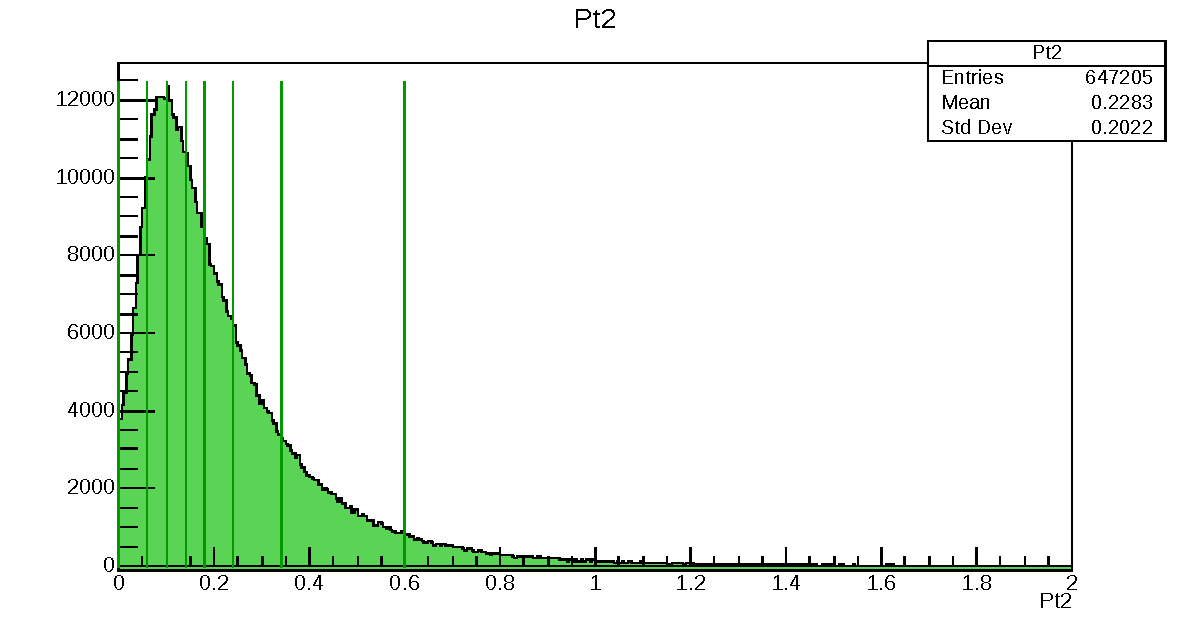
\includegraphics[width=\linewidth]{13dataanalysis/img/40_accbins_pt2.pdf}
    %         % \caption{$P_T^2$ bins.}
    %         \label{fig::acc_corr_bins_pt2}
    %     \end{subfigure}
    %     \begin{subfigure}{.5\textwidth}
    %         \centering
    %         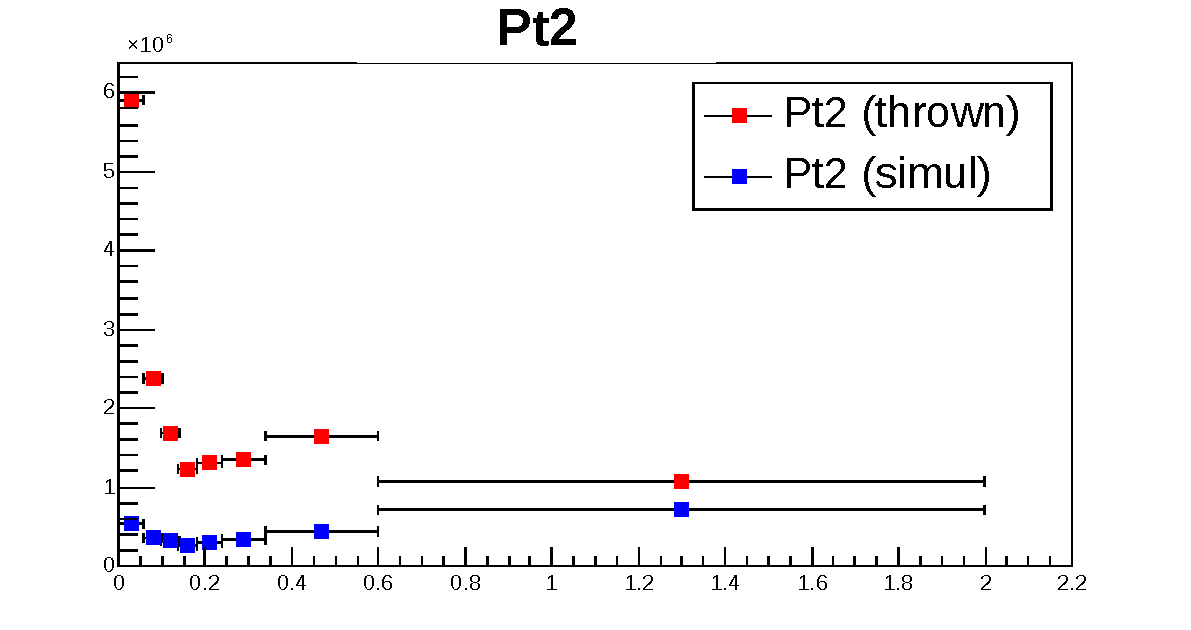
\includegraphics[width=\linewidth]{13dataanalysis/img/40_acccorr_pt2.pdf}
    %         % \caption{$P_T^2$ acceptance correction results.}
    %         \label{fig::acc_corr_pt2}
    %     \end{subfigure}
    %
    %     % phi_PQ.
    %     \begin{subfigure}{.5\textwidth}
    %         \centering
    %         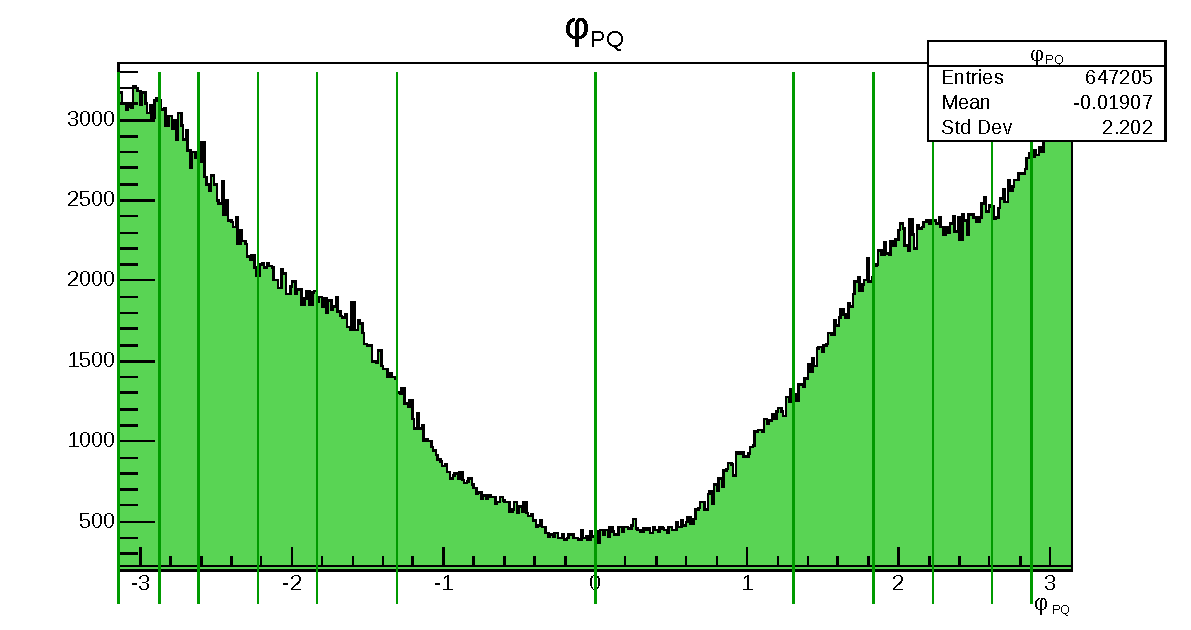
\includegraphics[width=\linewidth]{13dataanalysis/img/40_accbins_phipq.pdf}
    %         % \caption{$\phi_{PQ}$ bins.}
    %         \label{fig::acc_corr_bins_phipq}
    %     \end{subfigure}
    %     \begin{subfigure}{.5\textwidth}
    %         \centering
    %         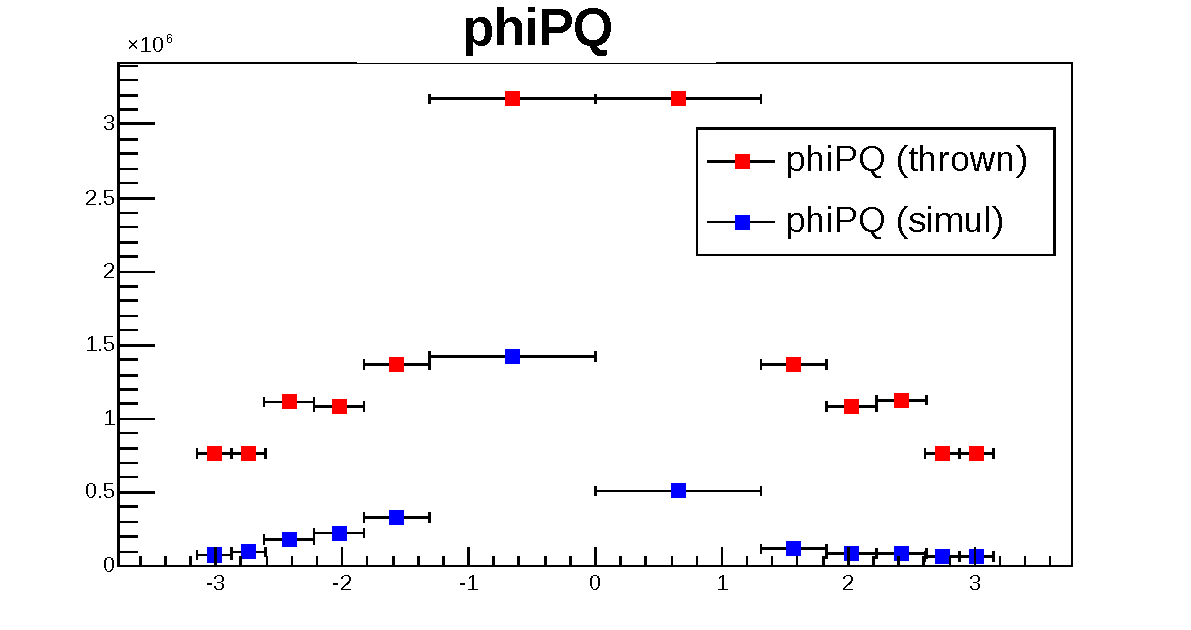
\includegraphics[width=\linewidth]{13dataanalysis/img/40_acccorr_phipq.pdf}
    %         % \caption{$\phi_{PQ}$ acceptance correction results.}
    %         \label{fig::acc_corr_phipq}
    %     \end{subfigure}
    %
    %     \caption[Acceptance correction results.]{Acceptance correction results for the kinematical variables $Q^2$, $\nu$, $z_h$, $p_T^2$, and $\phi_{PQ}$. On the left plots, the acceptance correction bin edges are shown. On the right, the number of thrown (in red) and simulated (in blue) entries for each of the variables is shown. All other variables are integrated for each plot.}
    %     \label{fig::acc_corr}
    % \end{figure}

    % !TEX root = ../main.tex
\subsection{Study Results}
\label{14.30::study_results}
    % TODO. Explain binning scheme selected.

    % TODO. Explain how "good" bins will be selected.
    %   * TODO. First criterium for selecting a good bin is maximising the phase space of each variable.
    %   * TODO. Then, the second criterium is maximising the statistics of that variable.
    %   * NOTE. As Hayk if I should use the results without acceptance correction to deduce the statistics?

    % statistical error estimation.
    The total statistical error on the acceptance corrected result $e_\text{corr}$ needs to consider both the statistical error of the measurements $e_\text{meas}$ and that of the acceptance correction $e_\text{acc}$.
    The former is purely statistical in nature, and is thus given by
    \begin{equation*}
        e_\text{meas} = \frac{\delta y_\text{meas}}{y_\text{meas}},
    \end{equation*}
    and the latter was derived in Equation \eqref{eq::14.20::acc_error}.

    Considering the fact that $e_\text{meas}$ comes purely from experimental data and $e_\text{acc}$ comes purely from simulation, they are completely uncorrelated.
    Thus, we can estimate the total statistical error of the acceptance corrected result as the quadratic addition of the two, or
    \begin{equation*}
        e_\text{corr} = \sqrt{e_\text{meas}^2 + e_\text{acc}^2}.
    \end{equation*}

    % TODO. systematic error "estimation".
    %   * TODO. Ask Raffaella for a reference about the "average" systematic error we should consider.

    % resulting plots.
    Each of the acceptance corrected DIS variables can be seen separated in $v_z$ bins in Figures \ref{fig::14.30::q2_vz} to \ref{fig::14.30::phipq_vz_-211}.
    The electron variables distributions, $Q^2$ and $\nu$, can be seen in Figures \ref{fig::14.30::q2_vz} and \ref{fig::14.30::nu_vz} respectively.
    Then, $z_h$ can be observed in Figures \ref{fig::14.30::zh_211_vz} for $e^-\pi^+$, and in \ref{fig::14.30::zh_-211_vz} for $e^-\pi^-$.
    $p_T^2$ for $e^-\pi^+$ can be seen in Figure \ref{fig::14.30::pt2_211_vz}, and for $e^-\pi^-$ in Figure \ref{fig::14.30::pt2_-211_vz}.
    At last, the $\phi_{PQ}$ distributions for $e^-\pi^+$ can be observed in Figure \ref{fig::14.30::phipq_211_vz}, while for $e^-\pi^-$ in Figure \ref{fig::14.30::phipq_-211_vz}.

    % Q2.
    \begin{figure}
        \centering
        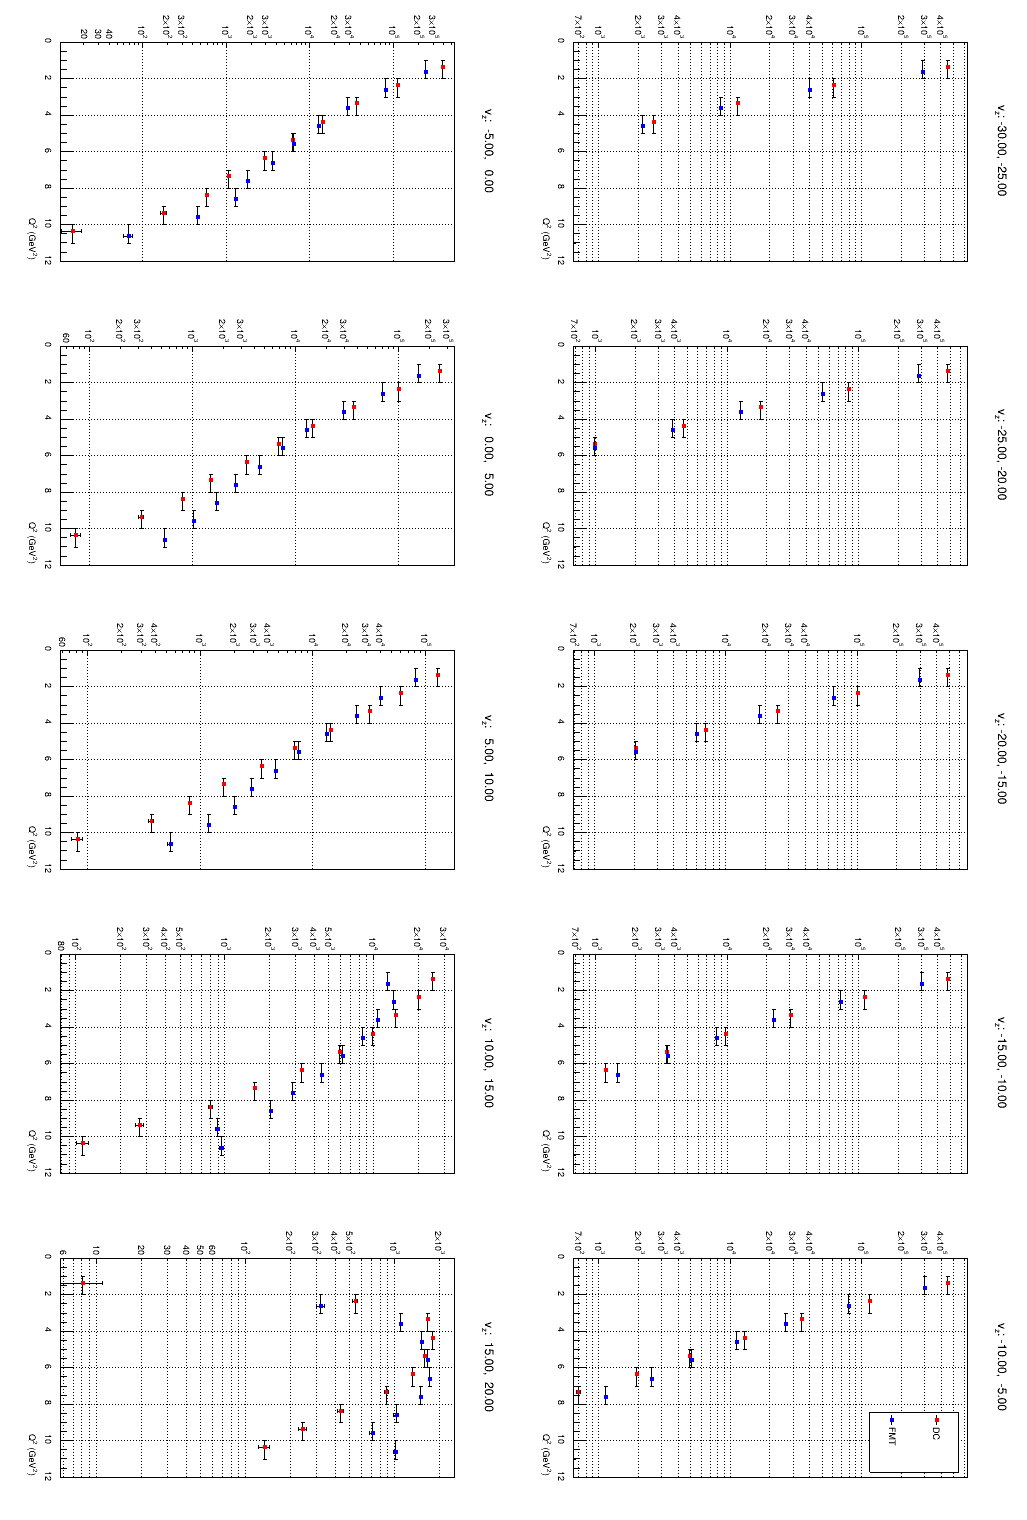
\includegraphics[width=\textwidth]{30q2_vz.png}
        \caption[Acceptance-corrected $Q^2$ separated in $v_z$ bins, run 12016]
        {Acceptance-corrected $Q^2$ detected by DC and FMT, separated in $v_z$ bins.
        Run 12016.}
        \floatfoot{Source: Own elaboration, using the \href{https://github.com/bleaktwig/clas12-rge-analysis}{clas12-rge-analysis} software.}
        \label{fig::14.30::q2_vz}
    \end{figure}

    % nu.
    \begin{figure}
        \centering
        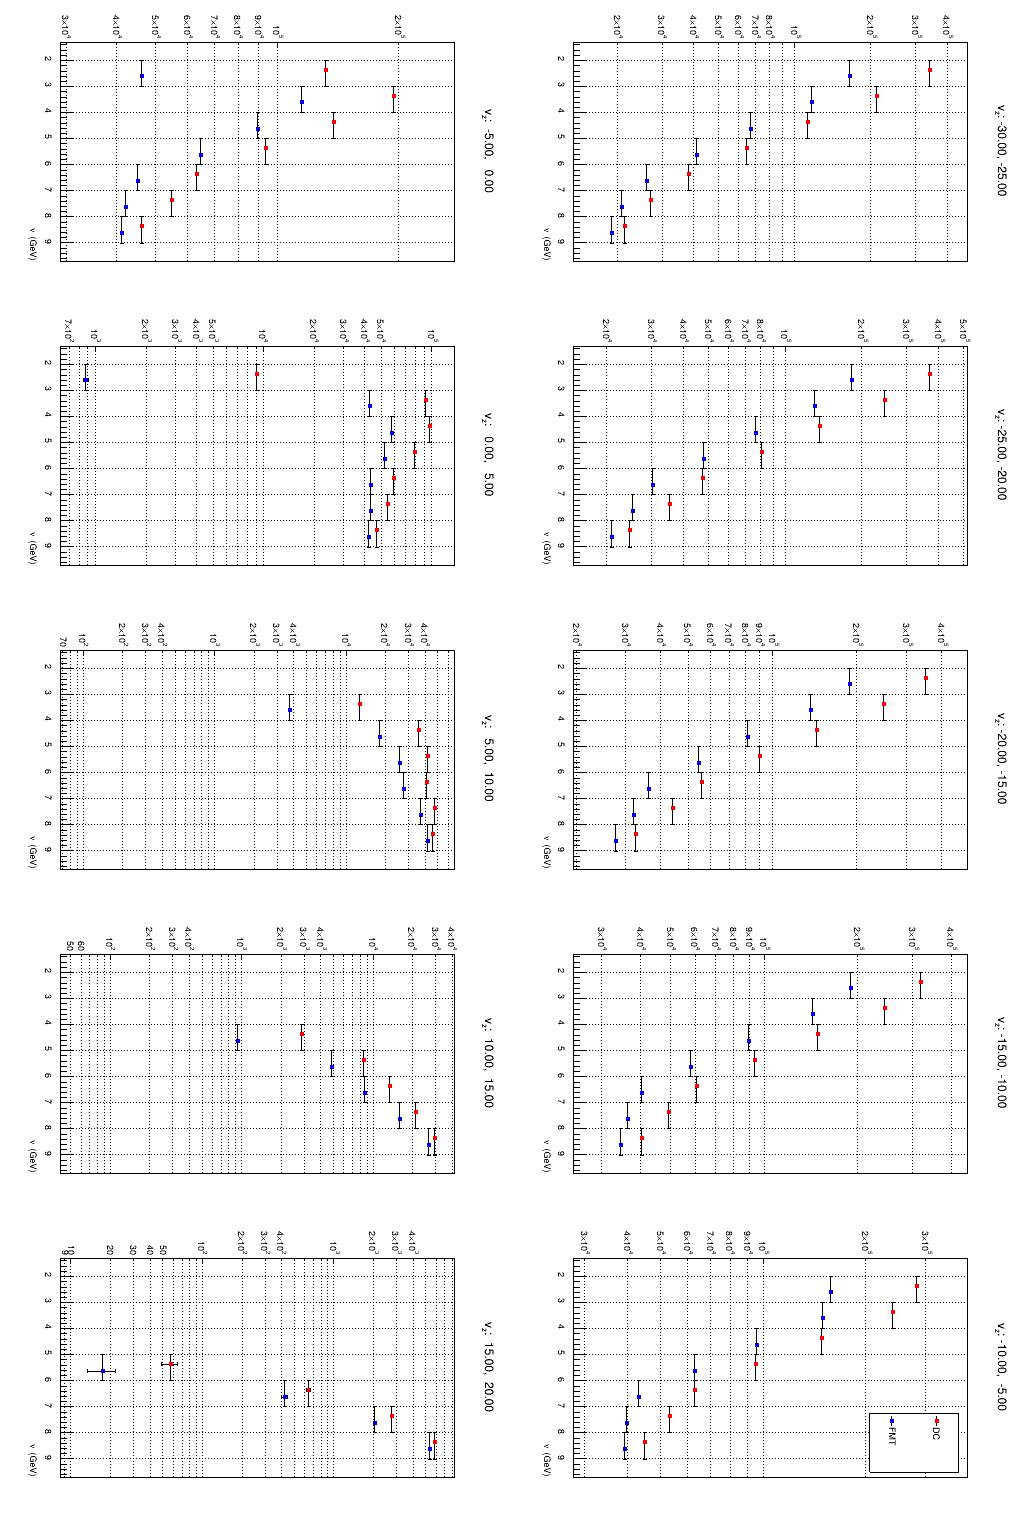
\includegraphics[width=\textwidth]{30nu_vz.png}
        \caption[Acceptance-corrected $\nu$ separated in $v_z$ bins, run 12016]
        {Acceptance-corrected $\nu$ detected by DC and FMT, separated in $v_z$ bins.
        Run 12016.}
        \floatfoot{Source: Own elaboration, using the \href{https://github.com/bleaktwig/clas12-rge-analysis}{clas12-rge-analysis} software.}
        \label{fig::14.30::nu_vz}
    \end{figure}

    % zh.
    \begin{figure}
        \centering
        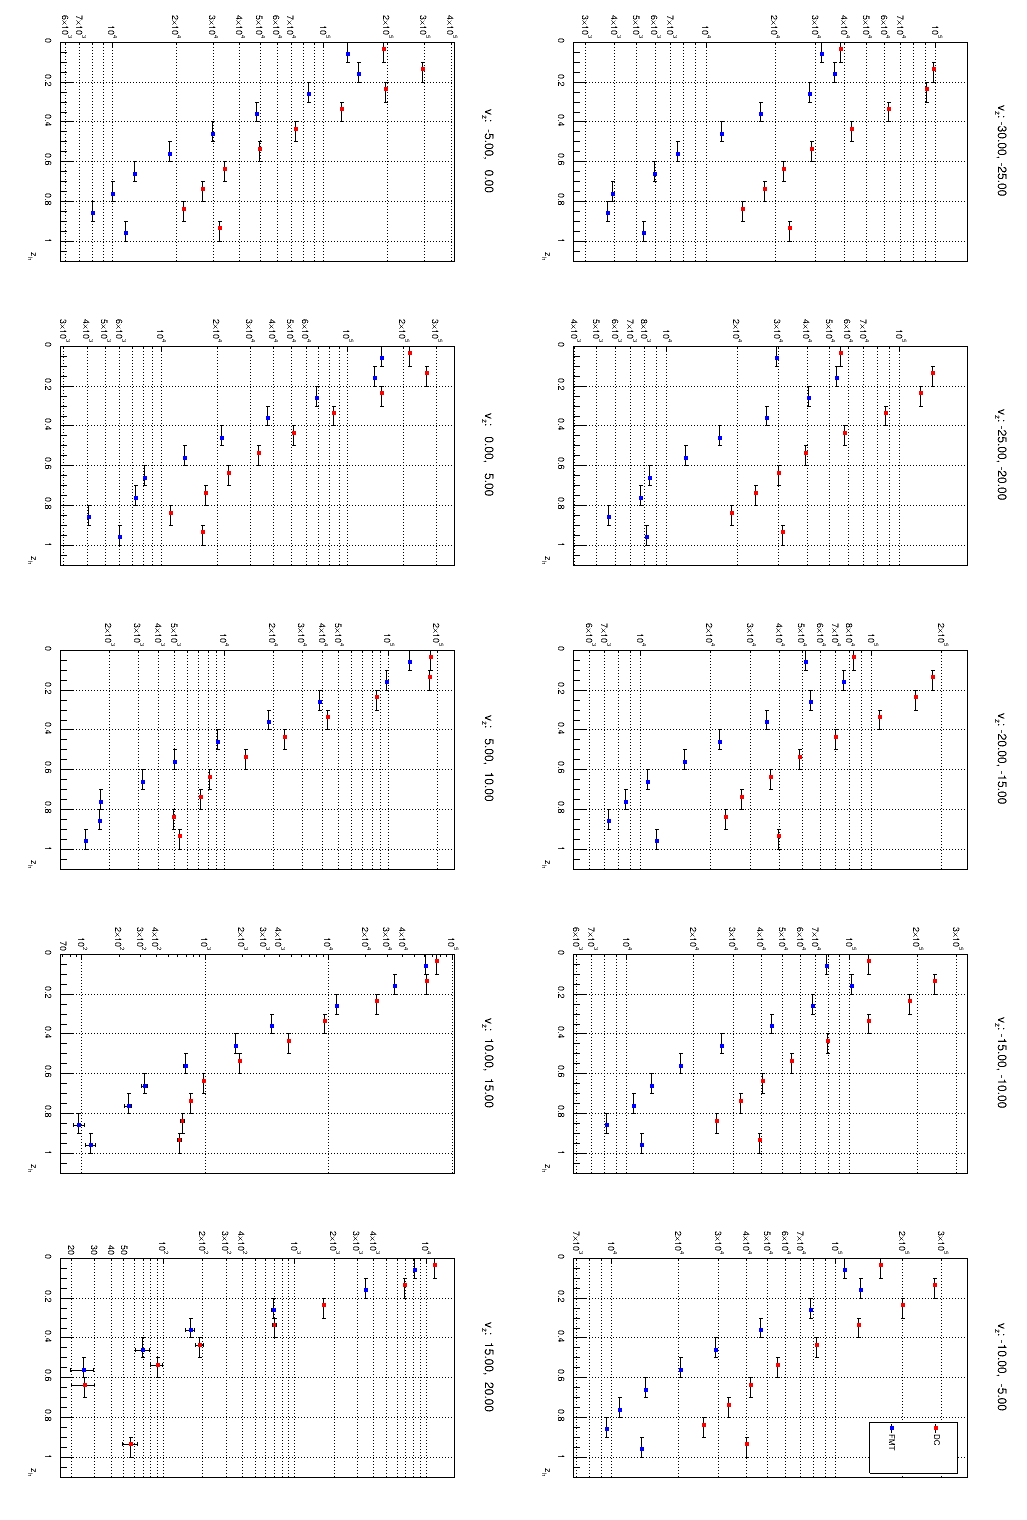
\includegraphics[width=\textwidth]{30zh_vz_211.png}
        \caption[Acceptance-corrected $z_h$ for $e^-\pi^+$ separated in $v_z$ bins, run 12016]
        {Acceptance-corrected $z_h$ for $e^-\pi^+$ detected by DC and FMT, separated in $v_z$ bins.
        Run 12016.}
        \floatfoot{Source: Own elaboration, using the \href{https://github.com/bleaktwig/clas12-rge-analysis}{clas12-rge-analysis} software.}
        \label{fig::14.30::zh_211_vz}
    \end{figure}

    \begin{figure}
        \centering
        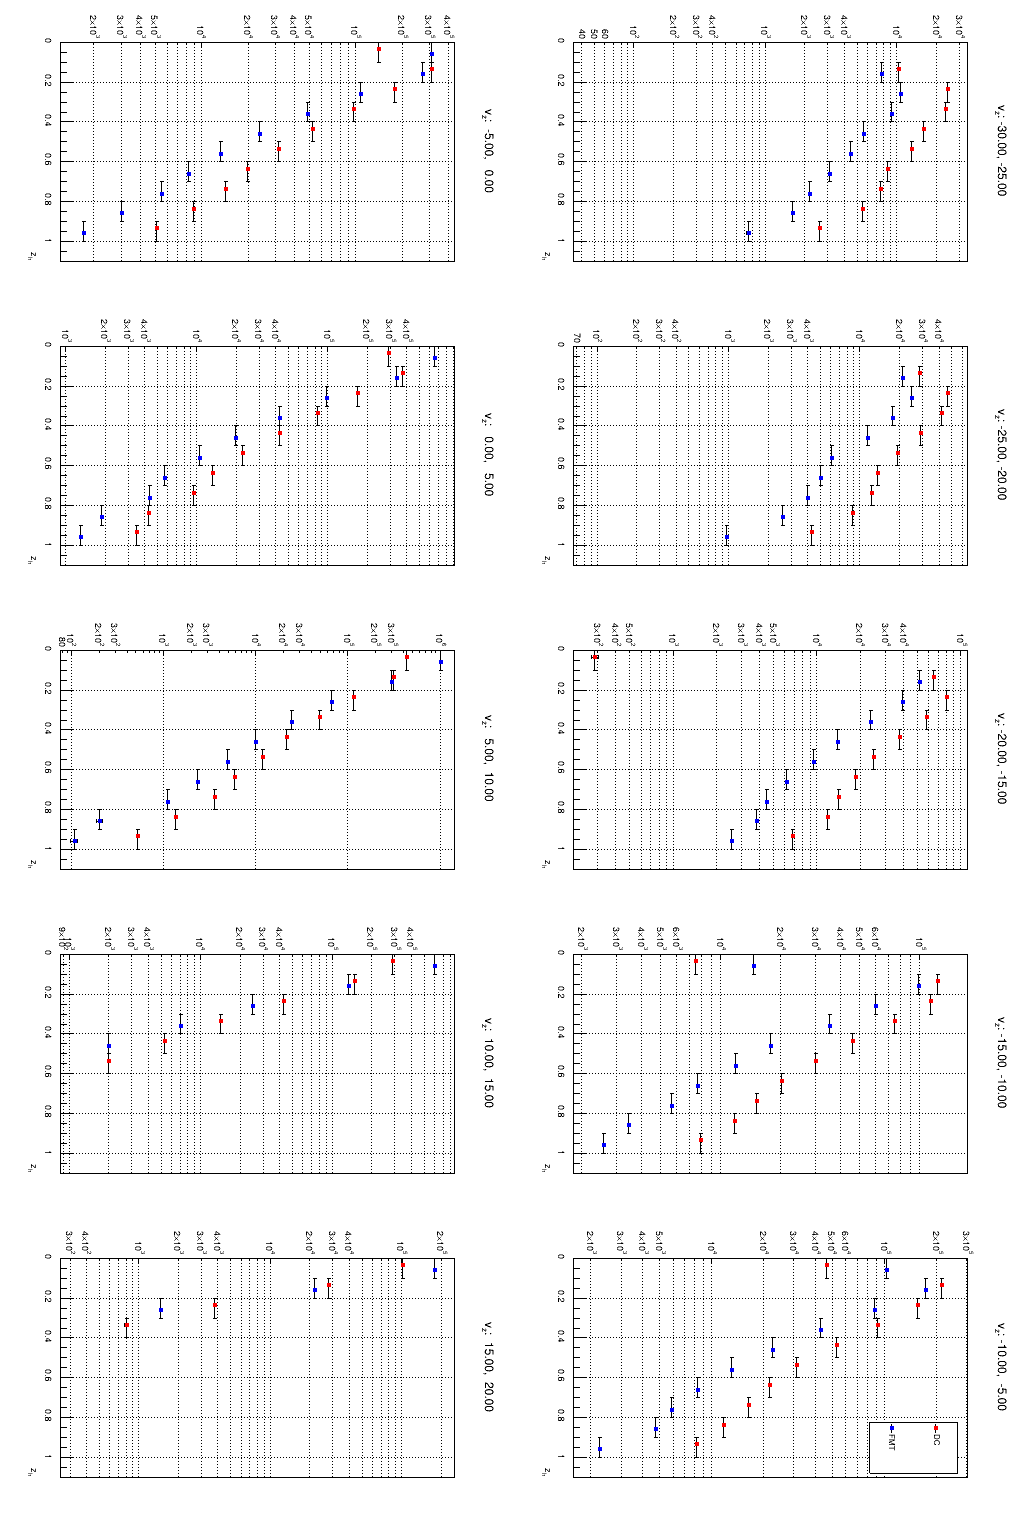
\includegraphics[width=\textwidth]{30zh_vz_-211.png}
        \caption[Acceptance-corrected $z_h$ for $e^-\pi^-$ separated in $v_z$ bins, run 12016]
        {Acceptance-corrected $z_h$ for $e^-\pi^-$ detected by DC and FMT, separated in $v_z$ bins.
        Run 12016.}
        \floatfoot{Source: Own elaboration, using the \href{https://github.com/bleaktwig/clas12-rge-analysis}{clas12-rge-analysis} software.}
        \label{fig::14.30::zh_-211_vz}
    \end{figure}

    % pt2.
    \begin{figure}
        \centering
        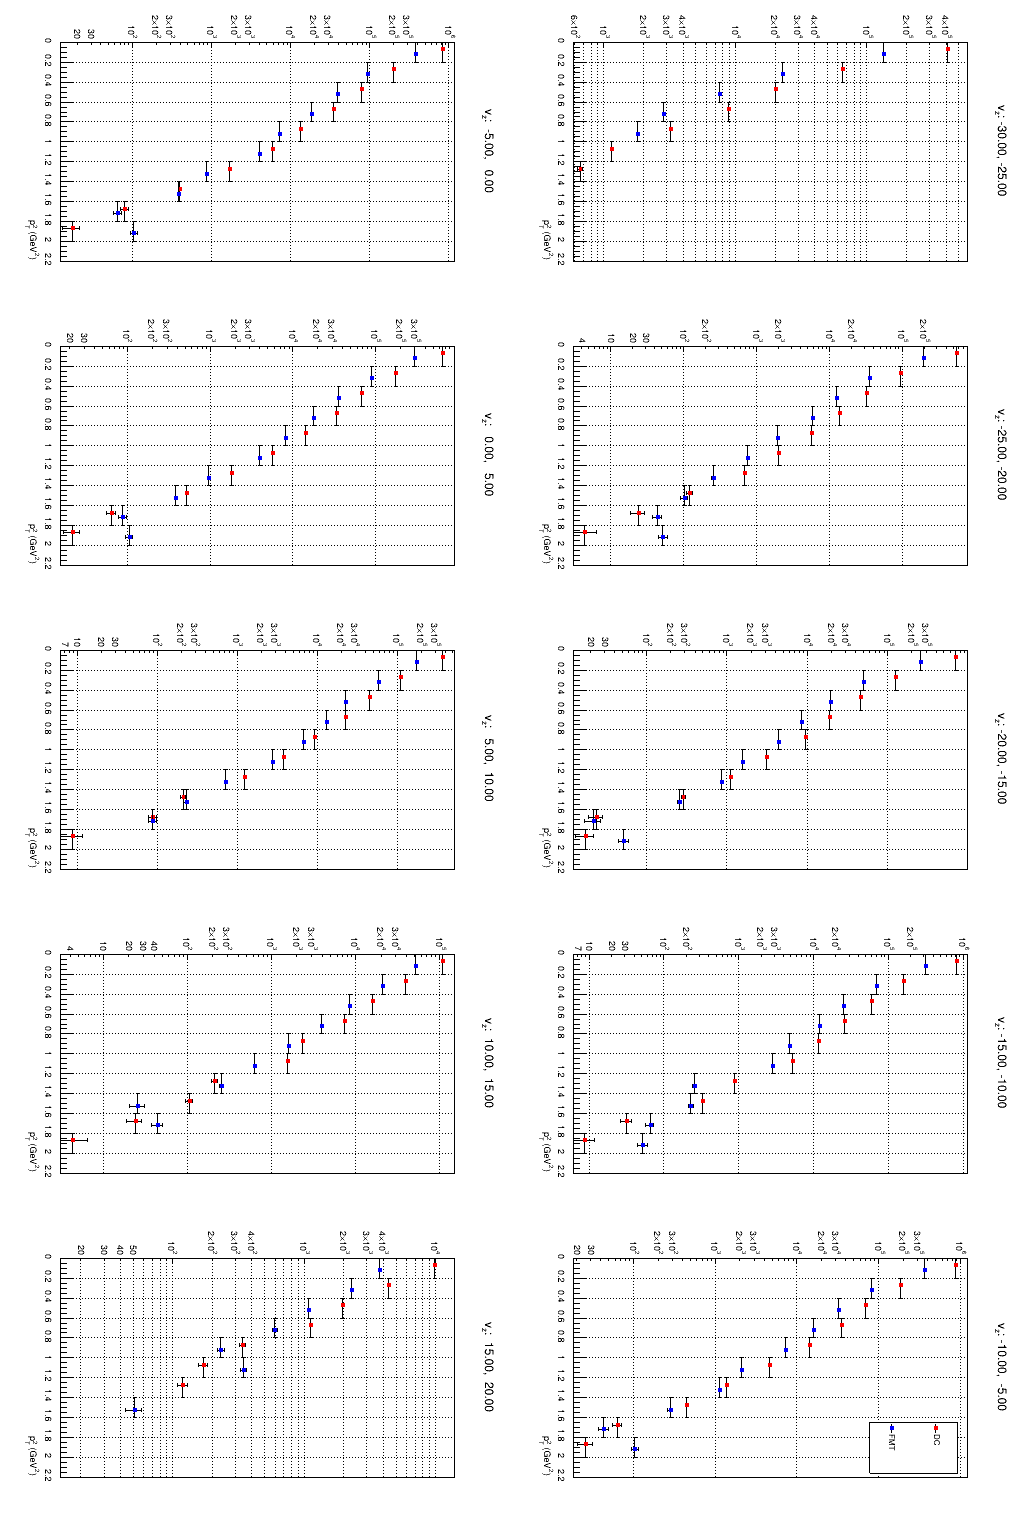
\includegraphics[width=\textwidth]{30pt2_vz_211.png}
        \caption[Acceptance-corrected $p_T^2$ for $e^-\pi^+$ separated in $v_z$ bins, run 12016]
        {Acceptance-corrected $p_T^2$ for $e^-\pi^+$ detected by DC and FMT, separated in $v_z$ bins.
        Run 12016.}
        \floatfoot{Source: Own elaboration, using the \href{https://github.com/bleaktwig/clas12-rge-analysis}{clas12-rge-analysis} software.}
        \label{fig::14.30::pt2_211_vz}
    \end{figure}

    \begin{figure}
        \centering
        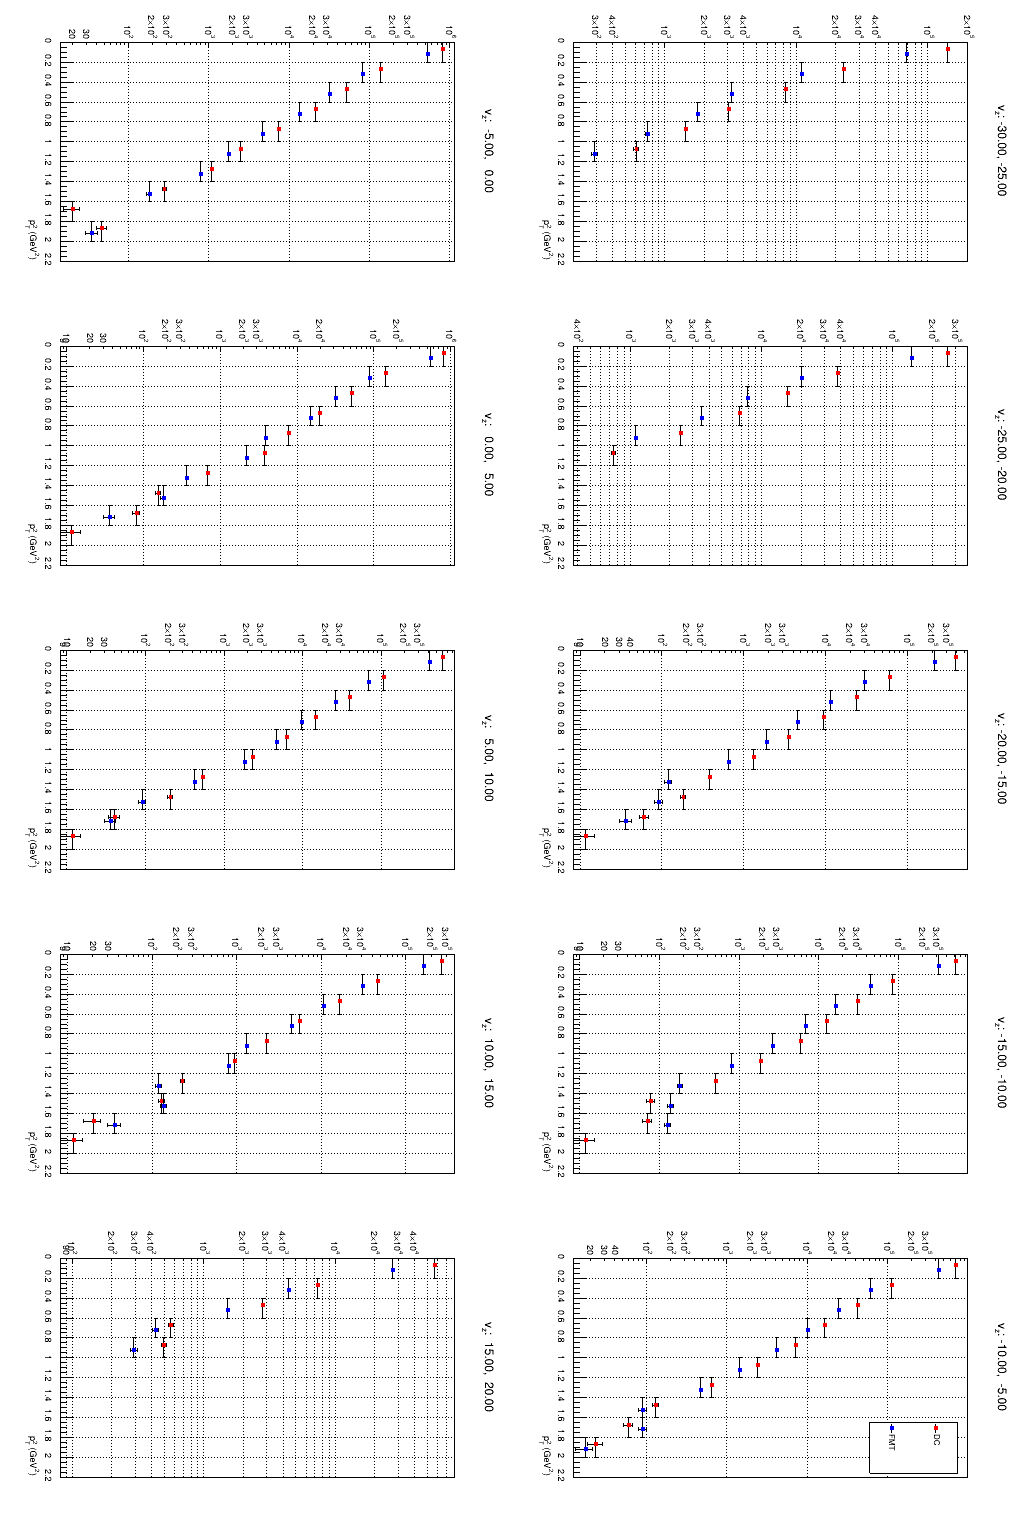
\includegraphics[width=\textwidth]{30pt2_vz_-211.png}
        \caption[Acceptance-corrected $p_T^2$ for $e^-\pi^-$ separated in $v_z$ bins, run 12016]
        {Acceptance-corrected $p_T^2$ for $e^-\pi^-$ detected by DC and FMT, separated in $v_z$ bins.
        Run 12016.}
        \floatfoot{Source: Own elaboration, using the \href{https://github.com/bleaktwig/clas12-rge-analysis}{clas12-rge-analysis} software.}
        \label{fig::14.30::pt2_-211_vz}
    \end{figure}

    % phipq.
    \begin{figure}
        \centering
        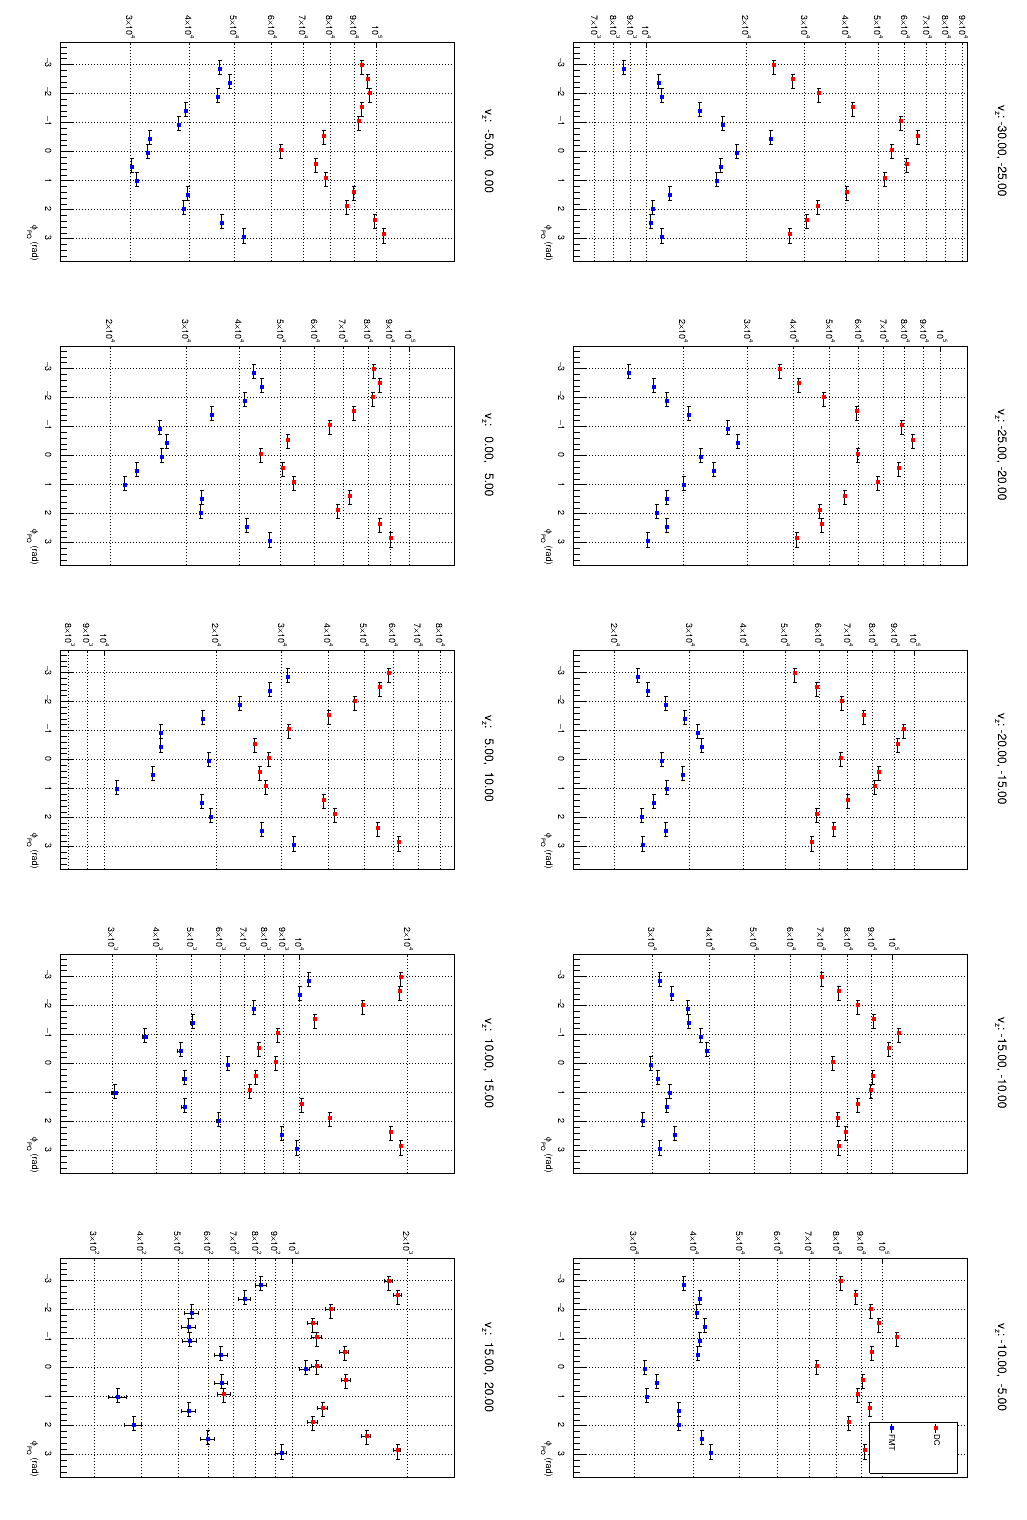
\includegraphics[width=\textwidth]{30phipq_vz_211.png}
        \caption[Acceptance-corrected $\phi_{PQ}$ for $e^-\pi^+$ separated in $v_z$ bins, run 12016]
        {Acceptance-corrected $\phi_{PQ}$ for $e^-\pi^+$ detected by DC and FMT, separated in $v_z$ bins.
        Run 12016.}
        \floatfoot{Source: Own elaboration, using the \href{https://github.com/bleaktwig/clas12-rge-analysis}{clas12-rge-analysis} software.}
        \label{fig::14.30::phipq_211_vz}
    \end{figure}

    \begin{figure}
        \centering
        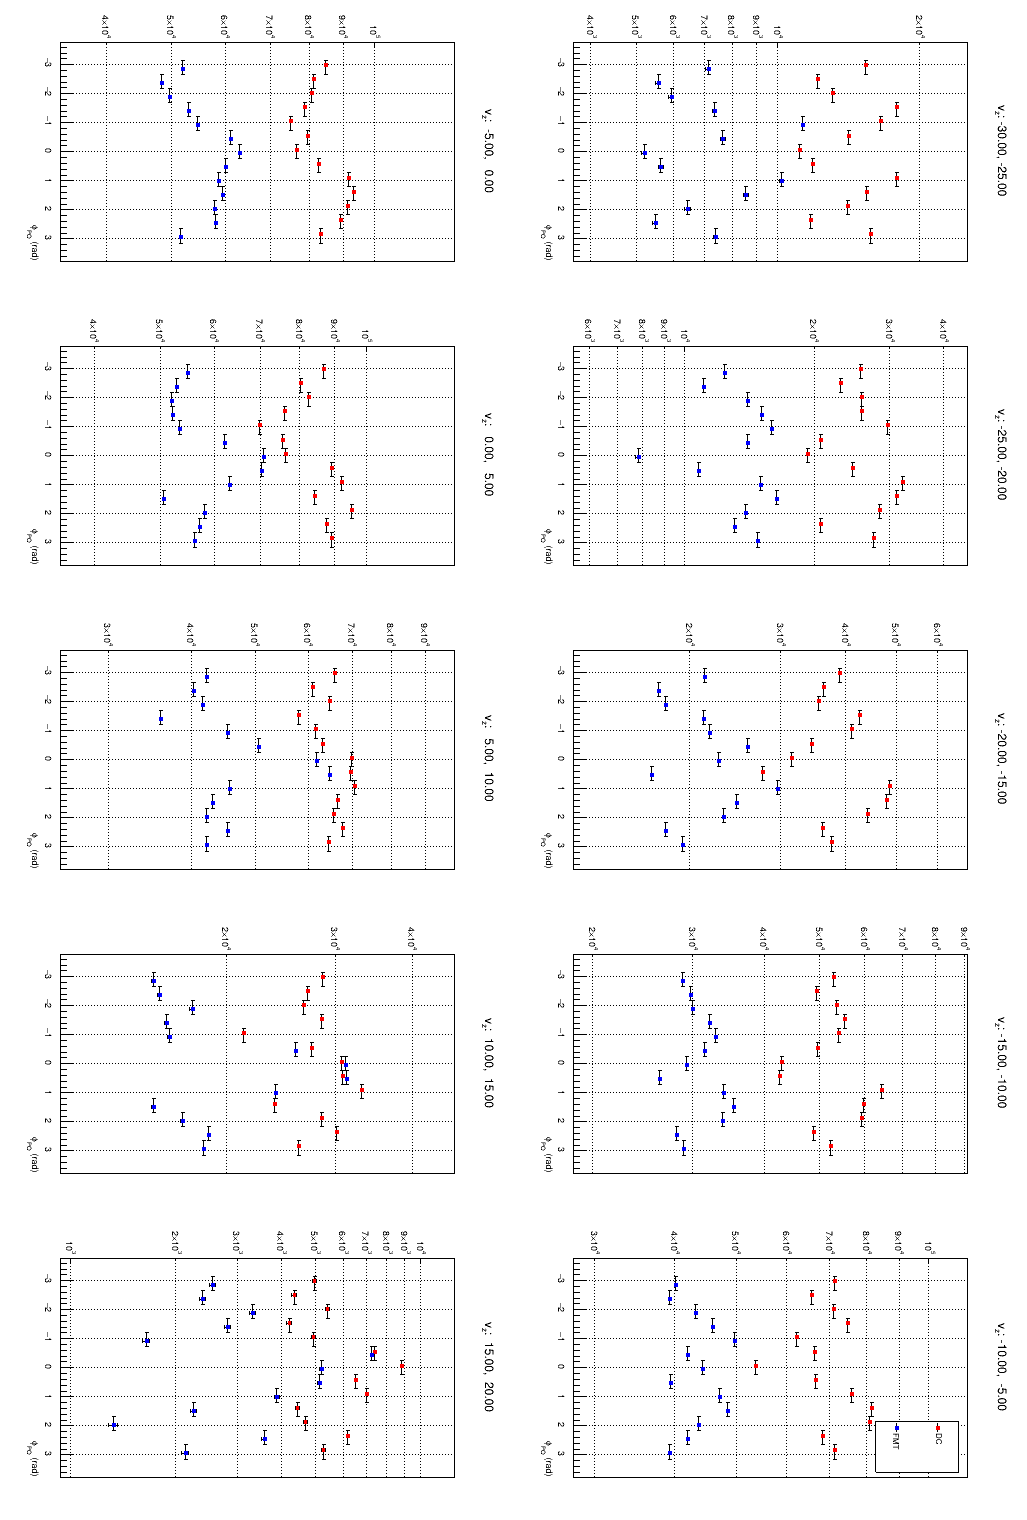
\includegraphics[width=\textwidth]{30phipq_vz_-211.png}
        \caption[Acceptance-corrected $\phi_{PQ}$ for $e^-\pi^-$ separated in $v_z$ bins, run 12016]
        {Acceptance-corrected $\phi_{PQ}$ for $e^-\pi^-$ detected by DC and FMT, separated in $v_z$ bins.
        Run 12016.}
        \floatfoot{Source: Own elaboration, using the \href{https://github.com/bleaktwig/clas12-rge-analysis}{clas12-rge-analysis} software.}
        \label{fig::14.30::phipq_-211_vz}
    \end{figure}

    % TODO. draw conclusions.

    % TODO. Mention nu and zh and how they shouldn't (and don't) show any dependence.

    % TODO. Metnion and show that Q2, pt2, and phiPQ show dependence on theta angle.

    % TODO. Decide on a range based on Q2 phase space. Show that the same can be concluded from pt2 and phiPQ, but Q2 is easier to study due to only coming from the e-.
    As can be seen on the figure, the higher end of the variable's phase space is limited for $v_z < -5$ cm, with the effect becoming more pronounced the further upstream we go.
    This effect can be understood by compounding the $\theta$ efficiency for negative particles (see Figure \ref{fig::14.21::theta_study_neg}) and the limited acceptance region of FMT given by Equation \eqref{eq::12.42::fmt_geometry_cut} (see Figure \ref{eq::12.42::vz_vs_theta}): the higher end of $\theta$ becomes limited for lower $v_z$ values.

    With the stated objective of maximising the phase space of each variable, this draws us to set the minimum $v_z$ for the RG-E target to $-5$ cm.
    Furthermore, we can limit the maximum $v_z$ to $10$ cm, since the low values of $\theta$ become limited by the lower end of the FMT's acceptance region.

    % TODO. Decide on a final position based on statistics.

    % !TEX root = ../main.tex
\subsection{Conclusions}
    \label{14.40::conclusions}
    % TODO. Something something something.
    % TODO. Mention issue of large systematic errors (~10%) not considered in the work.
    %   * TODO. Ask Raffaella for a reference about the "average" systematic error I should consider.

